\cotefile{151}

% Scan is upside down; reading orientation is 180 degrees.
\scanpage{8}

\hrule
\begin{tabular}{p{.47\linewidth}p{.47\linewidth}}
\textbf{ACADEMIE D'AIX-MARSEILLE} & AVIGNON le 6 décembre 1990\\
\rule{3cm}{.4pt}&\\
\textbf{INSPECTION ACADEMIQUE} & Jacques ROUX, responsable\\
\textbf{DE VAUCLUSE}&départemental de l'Action\\
\rule{1cm}{.4pt}&Culturelle,\\[1em]
C.D.A.C.N°16&à\\[1em]
&M
\end{tabular}

\uline{OBJET} : Projets d'Action Educative Collège.\\
Année scolaire 1990/1991

L'attribution des aides aux P.A.E. se déroulera cette année en deux temps :

\begin{tabular}{l p{.72\linewidth}}
DECEMBRE & - instruction des dossiers\\
&par l'Inspection Académique\\[1em]
&propositions à la M.I.A.D.A.C.\\[1em]
JANVIER & - Monsieur le Recteur attribue\\
&une aide globalisée à Monsieur\\
&l'Inspecteur d'Académie.
\end{tabular}

Une commission se réunit vers le 15 janvier 1991, afin d'assurer la ventilation des aides au niveau du département. Je vous demanderai alors de participer à cette Commission.

P/L'Inspecteur d'Académie

% Ink signature below the typed closing.
\handwritten{\illegible{1}}
% Separate printed fragment clipped at the lower edge of the upright sheet.
\illegible{1}
\margin{7}

\scanpage{9}

\textbf{ACADEMIE D'AIX-MARSEILLE}\\
\rule{3cm}{.4pt}\\
\textbf{INSPECTION ACADEMIQUE}\\
\textbf{DE VAUCLUSE}\\
\rule{1cm}{.4pt}
\mspage{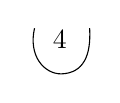
\begin{tikzpicture}[baseline=(n.base)]\node[inner sep=0pt] (n) at (0,0) {4};\draw (-.32,.15)..controls(-.4,-.2)and(-.2,-.43)..(.02,-.43)..controls(.3,-.42)and(.4,-.2)..(.38,.15);\end{tikzpicture}}
\[\begin{aligned}
p_{12}\delta_1(x)&=\sigma(x)\\
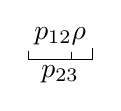
\begin{tikzpicture}[baseline=(t.base)]\node[inner sep=0pt] (t) {$p_{12}\rho$};\draw ([xshift=-2pt,yshift=-2pt]t.south west)--([xshift=-2pt,yshift=-5pt]t.south west)--([xshift=2pt,yshift=-5pt]t.south east)--([xshift=2pt,yshift=-1pt]t.south east);\draw ([xshift=4pt,yshift=-5pt]t.south)--++(0,2.5pt);\node[anchor=north,inner sep=0pt] at ([yshift=-7pt]t.south) {$p_{23}$};\end{tikzpicture}\delta_1(x)&=\delta_0p_0(x)\\
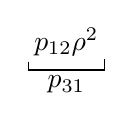
\begin{tikzpicture}[baseline=(t.base)]\node[inner sep=0pt] (t) {$p_{12}\rho^2$};\draw ([xshift=-2pt,yshift=-2pt]t.south west)--([xshift=-2pt,yshift=-5pt]t.south west)--([xshift=2pt,yshift=-5pt]t.south east)--([xshift=2pt,yshift=-1pt]t.south east);\node[anchor=north,inner sep=0pt] at ([yshift=-7pt]t.south) {$p_{31}$};\end{tikzpicture}\delta_1(x)&=x
\end{aligned}\]
\margin{NB $\delta_1(x)$ ne peut être fixe par $\rho$ (donc par $\unsure{\mathcal G_3|\mathfrak S_3}$) que si $x=\delta_0p_0(x)$ (condition néc. et suff.)}
\[\begin{tikzpicture}[baseline=(r.base)]
\node[inner sep=6pt] (r) {$\begin{gathered}\delta_0p_0(x)=1\\\sigma(x).x=1\\[.5em]p_{12}(z)p_{23}(z)p_{31}(z)=1\end{gathered}$};
\draw ([xshift=3pt,yshift=2pt]r.north west)--([xshift=-3pt,yshift=2pt]r.north east);
\draw ([yshift=-2pt]r.north west)--(r.south west)--(r.south east)--([yshift=-2pt]r.north east);
\end{tikzpicture}\]
\[\sigma(x)\begin{tikzpicture}[baseline=(t.base)]\node[inner sep=0pt] (t) {$\delta_0p_0(x)$};\draw ([xshift=-2pt,yshift=-2pt]t.south west)--([xshift=-2pt,yshift=-5pt]t.south west)--([xshift=2pt,yshift=-5pt]t.south east)--([xshift=2pt,yshift=-1pt]t.south east);\node[anchor=north,inner sep=0pt] at ([yshift=-7pt]t.south) {$\substack{\Vert\\1}$};\end{tikzpicture}x=1\]
pour $z\in E_2$ (une relation \deleted{\unsure{par|pour}} supplémentaire par orbite 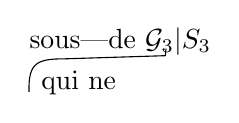
\begin{tikzpicture}[baseline=(w.base)]
\node[anchor=west,inner sep=0pt] (w) at (0,0) {qui ne};
\node[anchor=west,inner sep=0pt] at (-.15,.52) {\inserted{\unsure{sous|de} $\unsure{\mathcal G_3|\mathfrak S_3}$}};
\draw (-.15,-.12)..controls(-.16,.25)and(-.05,.3)..(.3,.3)--(1.58,.34)--(1.59,.43);
\end{tikzpicture} rencontre pas $\delta_1(E_1)$)
\diagram{\begin{tikzpicture}[x=1cm,y=1cm]
\node at (-.6,0) {$\delta_1$};
\node (top) at (1.8,0) {$F\times F\times F$};
\node at (1.8,1.45) {$\sigma_1$};
\draw (1.53,.63)..controls(1.15,.9)and(1.72,1.37)..(2.13,1.16)..controls(2.6,.96)and(2.24,.68)..(2.05,.61);
\draw (1.53,.63)--(1.58,.68);\draw (2.05,.61)--(2.01,.74);
\draw[line width=.7pt] (1.58,-.42)..controls(1.52,-.3)and(1.56,-.95)..(1.58,-1.12);
\draw[line width=.7pt] (1.46,-1.01)--(1.58,-1.12)--(1.7,-1.02);
\node at (1.08,-.7) {$p_{12}$};
\draw[line width=.7pt] (2.14,-.37)..controls(2.03,-.25)and(2.08,-.93)..(2.13,-1.1);
\draw (2.13,-1.1)--(2.12,-.31)--(2.29,-.44);
\draw[line width=.7pt] (2,-.98)--(2.13,-1.1)--(2.28,-.99);
\node at (2.7,-.7) {$p_{13}$};
\draw (top.east)..controls(4.1,.24)and(6,.38)..(8.2,.4);
\draw (4.13,-.03)..controls(5.65,.37)and(6.9,.17)..(7.53,.18)--(7.48,.27);
\node at (6.5,-.9) {$\alpha\in E_1$};
\node at (-.2,-1.7) {$F_\alpha$};\node at (.7,-1.7) {$\subset$};
\node at (1.8,-1.7) {$F\times F$};
\draw (1.83,-2.08)--(1.86,-2.95);\draw (1.72,-2.82)--(1.86,-2.95)--(2,-2.83);
\node at (2.36,-2.45) {$\mathrm{pr}_0$};\node at (1.86,-3.25) {$F$};
\end{tikzpicture}}
\[(x,y)\mapsto y\]
\[(x,y)\times_{\unsure{y|x}}\unsure{x'|x^+},y')\sim(x,\deleted{y},y')\]
\[\Pi_0(F_\alpha\times_F F_\alpha)=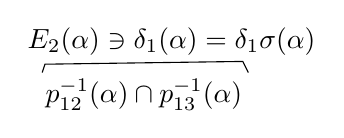
\begin{tikzpicture}[baseline=(t.base)]
\node[inner sep=0pt] (t) {$p_{12}^{-1}(\alpha)\cap p_{13}^{-1}(\alpha)$};
\draw ([xshift=-1pt,yshift=2pt]t.north west)--([xshift=0pt,yshift=5pt]t.north west)--([xshift=0pt,yshift=6pt]t.north east)--([xshift=2pt,yshift=2pt]t.north east);
\node[anchor=south,inner sep=0pt] at ([xshift=10pt,yshift=8pt]t.north) {$E_2(\alpha)\ni\delta_1(\alpha)=\delta_1\sigma(\alpha)$};
\end{tikzpicture}\qquad\text{stable par }\sigma_1\]
\margin{Le petit coq aux champs\\\deleted{\unsure{tél}}\\$\boxed{32\ 41\ 04\ 19}$}
\margin{$y,x,y$}
Prenons $\alpha\ne\delta_1$, alors $\delta_2\notin p_{12}^{-1}(\alpha)$

les p\textsuperscript{ts} fixes par $\sigma_1$ sont dans image $\delta_1(E_1)$, mais $p_{12}(\delta_1(x))=p_{13}(\delta_1(x))=\sigma x$, donc \deleted{\unsure{il faut}}
\deleted{\unsure{faut} $\sigma x={}$} $\delta_1(x)\in E_2(\alpha)\Longleftrightarrow\overset{!}{\sigma}x=\alpha$ i.e. $x=\uline{\sigma\alpha}$

et $\uline{\delta_1\sigma}(\alpha)$ joue le rôle de $\delta_2=\delta_1(\alpha)$
\margin{8}

\scanpage{11}
\mspage{1}

Hyperrecouvrements.

Soit $\mathcal X$ une catégorie $\mathcal U$-topos. On veut définir \deleted{\unsure{une}} la notion d'\uline{hyperrecouvrement} de $\mathcal X$ (ou encore, du topos défini par $\mathcal X$), indexé par une petite catégorie $A$. \deleted{Un tel hyp} Ce sera par définition un foncteur
\diagram{\begin{tikzcd}[ampersand replacement=\&,row sep=small]
\varphi:\quad A\arrow[r]\&\mathcal X\\
\alpha\arrow[r,mapsto]\&U_\alpha\ (=\unsure{\varphi|\varphi_{\mathcal X}}(\alpha))
\end{tikzcd}}
, satisfaisant certaines conditions, inspirées par \unsure{le|la} 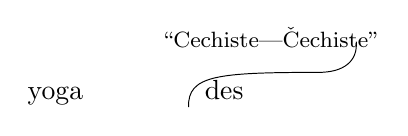
\begin{tikzpicture}[baseline=(yogab.base),x=1cm,y=1cm]
\node[anchor=base west,inner sep=0pt] (yogab) at (0,0) {yoga};
\node[anchor=base west,inner sep=0pt] at (2.25,0) {des};
\node[anchor=base west,inner sep=0pt,font=\footnotesize] at (1.70,.66) {\inserted{``\unsure{Cechiste|\v{C}echiste}''}};
\draw[line width=.35pt] (2.05,-.10) .. controls (2.04,.30) and (2.40,.34) .. (3.70,.34)
 .. controls (4.02,.34) and (4.20,.48) .. (4.18,.73);
\end{tikzpicture} recouvrements \unsure{et de} leurs nerfs, et le raffinement de ce y.g. suggéré par Cartier (pour les espaces topologiques non paracompacts). Voici les conditions qui me viennent à l'esprit:

\uline{Hyp 1} Les objets $U_\alpha$ ($\alpha\in\mathrm{Ob}\,A$) recouvrent l'\unsure{objet|objt} final $e_{\mathcal X}$ de $\mathcal X$.

\deleted{\uline{Hyp 1'} Pour tout $\alpha_0\in\mathrm{Ob}\,A$, le foncteur induit $A/\alpha_0\longrightarrow\mathcal X/U_{\alpha_0}$ satisfait à Hyp 1, i.e. l'ens. des flèches $U_\alpha\longrightarrow U_{\alpha_0}$, associé aux flèches $\alpha\longrightarrow\alpha_0$ de but $\alpha_0$ dans $A$,}
\margin{Est satisfait tautologiquement!}
\margin{10}

\scanpage{12}
\mspage{2}

reste couvrant.

\uline{Hyp 2}\unsure{a|.} Pour $\alpha,\beta\in\mathrm{Ob}\,A$, l'ens des \deleted{flèches} diagrammes
\diagram{\begin{tikzcd}[ampersand replacement=\&,column sep=small,row sep=small]\&\alpha\\\gamma\arrow[ur]\arrow[dr]\&\\\&\beta\end{tikzcd}}
dans $A$ (i.e. l'ens. des objets de $A_{/\alpha\times\beta}$, où $\alpha\times\beta$ est le produit cartésien dans $\widehat A$), indexant les flèches correspondantes $U_\gamma\longrightarrow U_\alpha\times U_\beta$, donne une famille \unsure{couvrante|couvrant} $U_\alpha\times U_\beta$.

[Idem pour une suite finie \inserted{(non vide)} $\alpha_0,\alpha_1,\ldots,\alpha_n$ ($n\in\mathbb N^{\deleted{\unsure{*}}}$) d'objets de $A$, et les \deleted{diagr.} flèches
\[U_\gamma\longrightarrow U_{\alpha_0}\times U_{\alpha_1}\times\cdots\times U_{\alpha_n}\]
indexées par les objets de $A_{/\alpha_0\times\alpha_1\times\cdots\alpha_n}$.]
\margin{[Hyp. 2 généralisé\unsure{.|:}]}

Pour $n=0$, on retrouve Hyp 1', pour $n=1$, la formulation initiale de Hyp 2. Mais Hyp 2 pour $n=1$ implique-t-il Hyp 2 pour \deleted{$\unsure{n>1}$ \unsure{quelconque}} $n\geq1$\unsure{.|?} On voit qu'il en est ainsi, par récurrence, en utilisant le fait que la famille composée de deux familles couvrantes
\diagram{\begin{tikzcd}[ampersand replacement=\&,column sep=large]
U_{\gamma'}\arrow[r,"\varphi(v)"]\&U_\gamma\times U_{\alpha_{n+1}}\arrow[r,"\varphi(u)\times\mathrm{id}_{U_{\alpha_{n+1}}}"]\&(U_{\alpha_0}\times\cdots\times U_{\alpha_n})\times U_{\alpha_{n+\unsure{1}}}
\end{tikzcd}}
($v$ parcourant les flèches $\gamma'\longrightarrow\gamma\times\alpha_{n+1}$, et $u$ les flèches \unsure{.} $\gamma\longrightarrow\alpha_0\times\cdots\times\alpha_n$) est couvrante. Ainsi Hyp 1' \deleted{\unsure{implique}} \inserted{$+$} Hyp 2\unsure{a|.}
\margin{11}

\scanpage{13}
\mspage{3}

forme initiale (cas $\alpha,\beta$) implique Hyp. 2 sous sa forme générale (en termes de $\alpha_0,\alpha_1,\ldots\alpha_n$).

\uline{Hyp.} 2': Pour tout $\alpha_0\in\mathrm{Ob}\,A$, le foncteur induit $A_{/\alpha_0}\unsure{\xrightarrow{\varphi}|\twoheadrightarrow|\longrightarrow}\mathcal X_{/\alpha_0}$ satisfait \unsure{à|:} Hyp 2 i.e. pour tout diagramme
\diagram{\begin{tikzcd}[ampersand replacement=\&,column sep=small,row sep=small]
\alpha_1\arrow[dr]\&\&\alpha_2\arrow[dl]\\
\&\alpha_0\&
\end{tikzcd}}
, regardant les carrés commutatifs dans $A$ qui le complètent en
\diagram{\begin{tikzcd}[ampersand replacement=\&,column sep=small,row sep=small]
\&\gamma\arrow[dl]\arrow[dr]\&\\
\alpha_1\arrow[dr]\&\&\alpha_2\arrow[dl]\\
\&\alpha_0\&
\end{tikzcd}}
, i.e. les objets de $A_{/\alpha_1\times_{\alpha_0}\alpha_2}$, la famille des flèches correspondantes
\[U_\gamma\longrightarrow U_{\alpha_1}\times_{U_{\alpha_0}}U_{\alpha_2}\]
est couvrante (i.e., épimorphique).

Les hypothèses Hyp 1, 2, 2' se reformulent joliment, en termes du prolongement canonique
\[\varphi_!:\widehat A\longrightarrow\mathcal X\]
de $\varphi$ en un foncteur 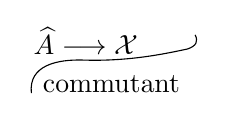
\begin{tikzpicture}[baseline=(w.base)]
\node[anchor=west,inner sep=0pt] (w) at (0,0) {commutant};
\node[anchor=west,inner sep=0pt] at (-.12,.54) {\inserted{$\widehat A\longrightarrow\mathcal X$}};
\draw (-.14,-.12)..controls(-.18,.24)and(.2,.31)..(.52,.3)..controls(1.12,.28)and(1.6,.39)..(1.84,.44)..controls(1.96,.48)and(1.98,.54)..(1.94,.62);
\end{tikzpicture} \deleted{\unsure{à|et}} aux petites $\lim_{\longrightarrow}$. Ce sont respectivement
\margin{12}

\scanpage{14}
\mspage{4}

\[
\text{a)}\quad \varphi_!(e_{\widehat A})\longrightarrow e_{\mathcal X}\quad\text{est épi}
\]
\[
\text{b)}\quad \varphi_!(\alpha\times\beta)\longrightarrow
\varphi_!(\alpha)\times\varphi_!(\beta)\quad\text{est épi}
\qquad \forall\alpha,\beta\text{ dans }\operatorname{Ob}A
\]
\[
\text{c)}\quad \varphi_!(\alpha\times_{\alpha_0}\beta)\longrightarrow
\varphi_!(\alpha)\times_{\varphi_!(\alpha_0)}\varphi_!(\beta)\quad\text{est épi}
\]
$\forall$ diagramme
\diagram{\begin{tikzcd}[ampersand replacement=\&,column sep=small,row sep=small]
\alpha\arrow[dr]\&\&\beta\arrow[dl]\\
\&\alpha_0\&
\end{tikzcd}}
dans $A$.

Un cas particulièrement agréable où ces conditions sont satisfaites, c'est quand $\varphi_!$ est exact à gauche, i.e. qu'il correspond \deleted{\unsure{à}} à un morphisme de topos
\[
f:\mathcal X\longrightarrow\widehat A
\]
par la formule
\[
\varphi_!=f^*.
\]
Alors dans a) b) c) les flèches épi en question sont même des iso, et je présume que l'inverse est vrai également. Oui -- et c'est essentiellement \unsure{evident|evid\textsuperscript{t}}, en écrivant canoniquement, pour un $F\in\operatorname{Ob}\widehat A$, $F=\varinjlim_{A/F}\alpha$ \unsure{$\ldots$}\unsure{.} On voit

\deleted{Mais \unsure{peut-on avoir}}
\inserted{de la $=$ façon pour} b) et c)

\margin{13}

\scanpage{15}
\mspage{5}

impliquent
\[
\text{b')}\quad\varphi_!(F\times G)\longrightarrow\varphi_!(F)\times\varphi_!(G)\quad\text{épi}
\qquad\forall F,G\text{ dans }\operatorname{Ob}\widehat A
\]
\[
\text{c')}\quad\varphi_!(G\times_F H)\longrightarrow
\varphi_!(G)\times_{\varphi_!(F)}\varphi_!(H)\quad\text{épi}
\]
$\forall$ diagramme
\diagram{\begin{tikzcd}[ampersand replacement=\&,column sep=small,row sep=small]
G\arrow[dr]\&\&H\arrow[dl]\\
\&F\&
\end{tikzcd}}
dans $\widehat A$.

et de là, plus généralement, la forme équivalente unique de Hyp 1, 2, 2' :

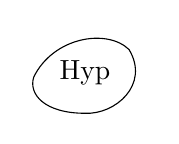
\begin{tikzpicture}[baseline=(n.base)]\node[inner sep=0pt] (n) at (0,0) {Hyp};\draw (-.65,-.05)..controls(-.4,.46)and(.28,.57)..(.56,.3)..controls(.83,-.15)and(.38,-.53)..(0,-.51)..controls(-.51,-.51)and(-.72,-.27)..(-.65,-.05);\end{tikzpicture}
Pour tout diagramme fini $(F_i)_{i\in I}$ dans $\widehat A$, la flèche canonique
\[
\varphi_!\left(\varprojlim_I F_i\right)\longrightarrow\varprojlim_I\varphi_!(F_i)
\]
est épi.

(Il suffit d'ailleurs de le postuler quand les $F_i$ sont dans $A$, et dans les trois cas particuliers $I=\bullet$, $\bullet\ \bullet$,
\diagram{\begin{tikzcd}[ampersand replacement=\&,column sep=tiny,row sep=tiny]
\bullet\arrow[dr]\&\&\bullet\arrow[dl]\\
\&\bullet\&
\end{tikzcd}}, correspondants aux axiomes Hyp 1, Hyp 2, Hyp $2'$.)

Mais cette hypothèse peut-elle être vérifiée, sans que $\varphi_!$ soit $=$ ex.\textsuperscript{t} à gauche ?

\margin{14}

% First reader C; scan 017 only. Unresolved notation is repeated in place.
\scanpage{17}
\mspage{\textcircled{1}}

\diagram{\begin{tikzcd}[ampersand replacement=\&]
\mathbb E_n\arrow[r,shift left,"{\unsure{\delta|\partial}}_n"]\&\mathbb E_{n+1}\arrow[l,shift left,"K_n"]
\end{tikzcd}}
$n\in\mathbb N^*\quad\text{i.e. }n\geq1$

\[
\left.\begin{aligned}
{\unsure{\delta|\partial}}_n &: [1,n]\hookrightarrow[1,n+1]&&\text{inclusion}\\
K_n &: [1,n]\longleftarrow[1,n+1]&&\text{rétraction}
\end{aligned}\right]
\]
\margin{$\unsure{\mathcal G_n|\mathfrak S_n}$ opère sur $\mathbb E_n$
\diagram{\begin{tikzcd}[ampersand replacement=\&]
\unsure{\mathcal G_n|\mathfrak S_n}\arrow[r,hook,"i_n"]\&\unsure{\mathcal G_{n+1}|\mathfrak S_{n+1}}
\end{tikzcd}}}

\margin{${\unsure{\delta|\partial}}_nK_n\overset{\text{déf}}{=}p_{n+1}$ (\unsure{projection|projecteur} dans $\mathbb E_{n+1}$, rétraction sur $\mathbb E_n\subset\mathbb E_{n+1}$}
\figure{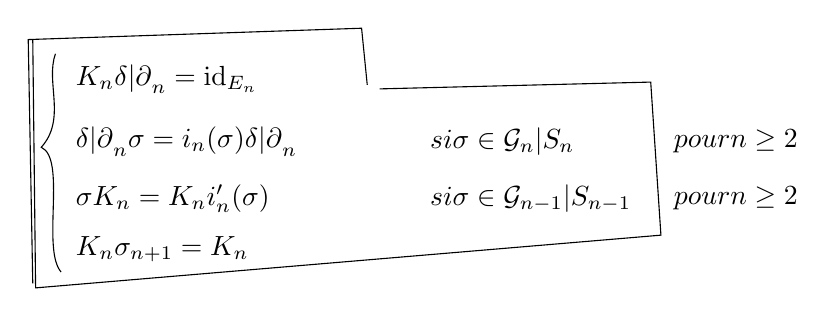
\begin{tikzpicture}[x=.72cm,y=.72cm]
\node[anchor=west,inner sep=0pt] at (0.75,3.2) {$K_n{\unsure{\delta|\partial}}_n=\mathrm{id}_{\mathbb E_n}$};
\node[anchor=west,inner sep=0pt] at (0.75,2.1) {${\unsure{\delta|\partial}}_n\sigma=i_n(\sigma){\unsure{\delta|\partial}}_n$};
\node[anchor=west,inner sep=0pt] at (0.75,1.1) {$\sigma K_n=K_n i^{\prime}_n(\sigma)$};
\node[anchor=west,inner sep=0pt] at (0.75,0.2) {$K_n\sigma_{n+1}=K_n$};
\node[anchor=west,inner sep=0pt] at (7,2.1) {$\text{si }\sigma\in\unsure{\mathcal G_{n}|\mathfrak S_{n}}$};
\node[anchor=west,inner sep=0pt] at (7,1.1) {$\text{si }\sigma\in\unsure{\mathcal G_{n-1}|\mathfrak S_{n-1}}$};
\node[anchor=west,inner sep=0pt] at (11.3,2.1) {$\text{pour }n\geq2$};
\node[anchor=west,inner sep=0pt] at (11.3,1.1) {$\text{pour }n\geq2$};
\draw (.4,3.65)..controls(.22,3.15)and(.6,2.5)..(.15,2.0)..controls(.6,1.8)and(.15,.2)..(.5,-.2);
\draw (0,-.4)--(-.08,3.9)--(5.8,4.1)--(5.9,3.1);
\draw (6.12,3.03)--(10.9,3.15)--(11.08,.45)--(.05,-.48)--(0,3.9);
\end{tikzpicture}}
\margin{où $i'_n\underset{\unsure{\text{déf}}}{=}i_n i_{n-1}:\unsure{\mathcal G_{n-1}|\mathfrak S_{n-1}}\longrightarrow\unsure{\mathcal G_n|\mathfrak S_n}\longrightarrow\unsure{\mathcal G_{n+1}|\mathfrak S_{n+1}}$}
\margin{où $\sigma_m\in\unsure{\mathcal G_m|\mathfrak S_m}$ est la transposition $[m-1,m)$}

\diagram{\begin{tikzcd}[ampersand replacement=\&]
\mathbb E_n^*\arrow[r,shift right=2,"d_n=K_n^*"']\&\mathbb E_{n+1}^*\arrow[l,shift right=2,"p_n={\unsure{\delta|\partial}}_n^*"']
\end{tikzcd}}

\figure{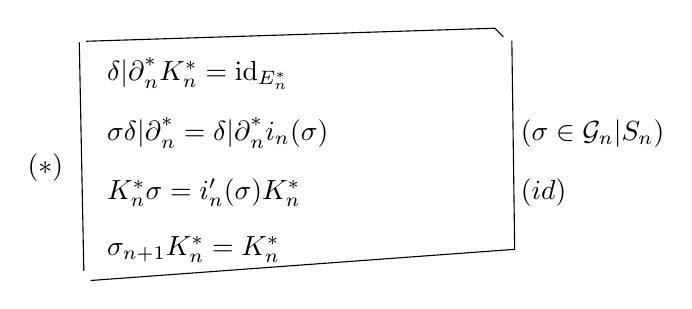
\begin{tikzpicture}[x=.72cm,y=.72cm]
\node[anchor=west,inner sep=0pt] at (-1,1.55) {$(*)$};
\node[anchor=west,inner sep=0pt] at (0.4,3.2) {${\unsure{\delta|\partial}}_n^*K_n^*=\mathrm{id}_{E_n^*}$};
\node[anchor=west,inner sep=0pt] at (0.4,2.15) {$\sigma{\unsure{\delta|\partial}}_n^*={\unsure{\delta|\partial}}_n^*i_n(\sigma)$};
\node[anchor=west,inner sep=0pt] at (0.4,1.1) {$K_n^*\sigma=i^{\prime}_n(\sigma)K_n^*$};
\node[anchor=west,inner sep=0pt] at (0.4,0.1) {$\sigma_{n+1}K_n^*=K_n^*$};
\node[anchor=west,inner sep=0pt] at (7.7,2.15) {$(\sigma\in\unsure{\mathcal G_{n}|\mathfrak S_{n}})$};
\node[anchor=west,inner sep=0pt] at (7.7,1.1) {$\text{(id)}$};
\draw (0,-.28)--(-.08,3.75);
\draw (.04,3.77)--(7.25,4.0)--(7.4,3.85);
\draw (7.55,3.78)--(7.6,.1)--(.12,-.45);
\end{tikzpicture}}
réalisation dans $(\mathrm{Ens})$ de syst. de
$(\text{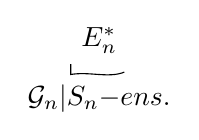
\begin{tikzpicture}[baseline=(e.base)]\node[inner sep=0pt] (e) at (0,0) {$E_n^*$};\draw (-.36,-.3)--(-.36,-.43)..controls(-.12,-.39)and(.12,-.48)..(.32,-.4);\node[anchor=north,inner sep=0pt] at (0,-.55) {$\unsure{\mathcal G_{n}|\mathfrak S_{n}}\text{-ens.}$};\end{tikzpicture}},{\unsure{\delta|\partial}}_n^*,K_n^*)$
satisfaisant aux relations $(*)$, \uline{plus}

\figure{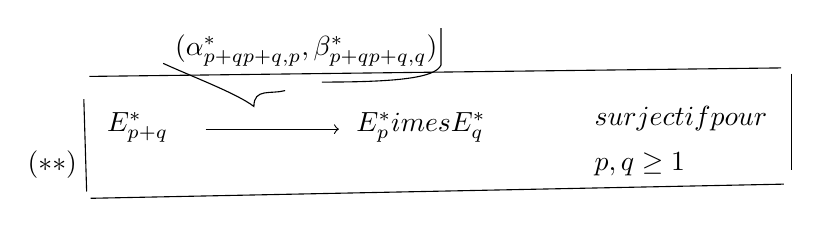
\begin{tikzpicture}[x=.72cm,y=.72cm]
\node[anchor=west,inner sep=0pt] at (-1,0.1) {$(**)$};
\node[anchor=west,inner sep=0pt] at (0.4,0.75) {$E_{p+q}^*$};
\node[anchor=west,inner sep=0pt] at (4.8,0.75) {$E_p^*	imes E_q^*$};
\node[anchor=west,inner sep=0pt] at (9,0.9) {$\text{surjectif pour}$};
\node[anchor=west,inner sep=0pt] at (9,0.1) {$p,q\geq1$};
\node[anchor=west,inner sep=0pt] at (1.6,2.1) {$\inserted{(\alpha^*_{\deleted{\unsure{p+q}}p+q,p},\beta^*_{\deleted{\unsure{p+q}}p+q,q})}$};
\draw[->] (2.15,.72)--(4.5,.72);
\draw (1.4,1.88)..controls(1.9,1.65)and(2.7,1.35)..(3.0,1.12)..controls(3.0,1.45)and(3.3,1.33)..(3.55,1.4);
\draw (4.2,1.55)..controls(5.5,1.55)and(6.2,1.62)..(6.3,1.85)--(6.3,2.5);
\draw (0,1.25)--(.05,-.38);
\draw (.1,1.65)--(12.3,1.8);
\draw (12.48,1.7)--(12.48,.0);
\draw (.12,-.5)--(12.35,-.25);
\end{tikzpicture}}

où
\[
\alpha^*_{n,p}:E_n^*\longrightarrow E_p^*\qquad(n>p\geq1)
\]
défini par
\[
\boxed{\alpha^*_{n,p}={\unsure{\delta|\partial}}_p^*{\unsure{\delta|\partial}}_{p+1}^*\cdots{\unsure{\delta|\partial}}_{n-1}^*}
\]
\diagram{\begin{tikzcd}[ampersand replacement=\&,column sep=small]
E_n^*\arrow[r,"{\unsure{\delta|\partial}}_{n-1}^*"]\&E_{n-1}^*\arrow[r,"{\unsure{\delta|\partial}}_{\unsure{n-2|n-1}}^*"]\&E_{n-2}^*\arrow[r]\&\cdots\arrow[r,"{\unsure{\delta|\partial}}_p^*"]\&E_p^*
\end{tikzcd}}

\[
\beta^*_{n,q}:E_n^*\longrightarrow E_q^*\qquad(n\geq q\geq1)
\]
défini par
\[
\boxed{\beta^*_{n,q}={\unsure{\delta|\partial}}_q^{\prime *}{\unsure{\delta|\partial}}_{q+1}^{\prime *}\cdots{\unsure{\delta|\partial}}_{n-1}^{\prime *}}
\]
\diagram{\begin{tikzcd}[ampersand replacement=\&,column sep=small]
E_n^*\arrow[r,"{\unsure{\delta|\partial}}_{n-1}^{\prime *}"]\&E_{n-1}^*\arrow[r,"{\unsure{\delta|\partial}}_{n-2}^{\prime *}"]\&E_{n-2}^*\arrow[r,phantom,"\cdots"]\&{}\arrow[r,"{\unsure{\delta|\partial}}_q^{\prime *}"]\&E_q^*
\end{tikzcd}}

avec ${\unsure{\delta|\partial}}_m^{\prime *}:E_{m+1}^*\longrightarrow E_m^*$ défini par
\[
\boxed{{\unsure{\delta|\partial}}_m^{\prime *}={\unsure{\delta|\partial}}_m^*\rho_{m+1}^*}
\]
\margin{$\rho_{m+1}^*=\rho_{m+1}^{-1}$ la permutation circu-\newline laire \unsure{élément.} inverse de $\unsure{\mathcal G_{m+1}|\mathfrak S_{m+1}}$}

\margin{$\alpha_{n,p}:\mathbb E_p\hookrightarrow\mathbb E_n$ inclusion canonique
\diagram{\begin{tikzcd}[ampersand replacement=\&,column sep=small]
\beta_{n,q}:\mathbb E_q\arrow[r,hook,no head]\&\mathbb E_n:\quad\beta_{n,q}(i)=i+(n-q)
\end{tikzcd}}
\[
{\unsure{\delta|\partial}}'_{\unsure{m|n}}:\mathbb E_{\deleted{\unsure{m+1}}m}\longrightarrow\mathbb E_{\deleted{\unsure{m}}m+1}
\qquad{\unsure{\delta|\partial}}'_n(i)=i+1
\]}
\[
\text{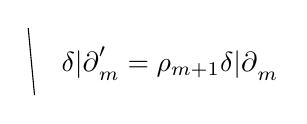
\begin{tikzpicture}[baseline=(e.base)]\node[inner sep=0pt] (e) at (0,0) {${\unsure{\delta|\partial}}'_m=\rho_{m+1}{\unsure{\delta|\partial}}_m$};\draw (-1.8,.45)--(-1.72,-.4);\end{tikzpicture}}
\]
où $\rho_m\in\unsure{\mathcal G_{m+1}|\mathfrak S_{m+1}}$ est la permutation circulaire
\[
\rho_m(i)=\begin{cases}i+1&\text{si }i\in[1,m],\\1&\text{si }i=m+1.\end{cases}
\]
\margin{16}

\scanpage{18}

\textbf{ACADEMIE D'AIX-MARSEILLE}\\
\rule{3cm}{.4pt}\\
\textbf{INSPECTION ACADEMIQUE}\\
\textbf{DE VAUCLUSE}\\
\rule{1cm}{.4pt}

\figure{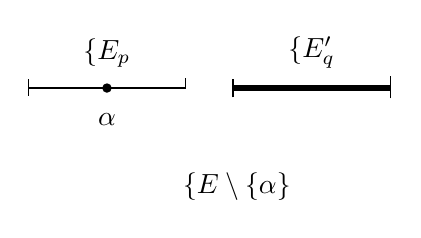
\begin{tikzpicture}[x=1cm,y=1cm]
\draw (0,0)--(2,0);\draw (0,-.10)--(0,.12);\draw (2,0)--(2,.13);\fill (1,0) circle (.06);
\node at (1,.45) {$\{E_p$};\node at (1,-.40) {$\alpha$};
\draw[line width=2pt] (2.6,0)--(4.6,0);\draw (2.6,-.12)--(2.6,.12);\draw (4.6,-.13)--(4.6,.15);
\node at (3.6,.45) {$\{E'_q$};
\node at (2.65,-1.25) {$\{E\setminus\{\alpha\}$};
\end{tikzpicture}}
\margin{$p\geq$}
\margin{278}

% Global cancellation is the manuscript's X, not a linewise sout.
\begingroup
\newsavebox{\SPXCIIICancelledXVIII}
\begin{lrbox}{\SPXCIIICancelledXVIII}
\begin{minipage}{\linewidth}

\[
\begin{gathered}
F=\varinjlim_{A/F}\alpha\\
G=\varinjlim_{A/G}\beta
\end{gathered}
\]

\[
\begin{aligned}
F\times G&=\varinjlim_{A/F}\text{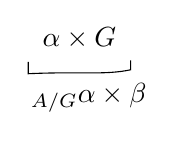
\begin{tikzpicture}[baseline=(e.base)]\node[inner sep=0pt] (e) at (0,0) {$\alpha\times G$};\draw (-0.65,-.3)--(-0.65,-.45)..controls(0,-.42)and(0.325,-.47)..(0.65,-.4)--(0.65,-.28);\node[anchor=north,inner sep=0pt] at (.12,-.57) {$\displaystyle \varinjlim_{A/G}\alpha\times\beta$};\end{tikzpicture}}\\
&=\varinjlim_{A/F\times A/G}\alpha\times\beta
\end{aligned}
\]

\par\noindent
\makebox[0pt][r]{%
  \smash{\begin{tabular}[t]{@{}l@{}}
  $\alpha\unsure{-|\longrightarrow}F$\\$\beta\unsure{-|\longrightarrow}G$
  \end{tabular}}\hspace{.75em}%
}\par

\figure{\begin{tikzpicture}[x=1cm,y=1cm]
\node[anchor=west] (prod) at (2.2,0) {$\displaystyle
\varphi_!(F\times G)=\varinjlim_{A/F\times A/G}
\text{\begin{tikzpicture}[baseline=(e.base)]\node[inner sep=0pt] (e) at (0,0) {$\varphi_!(\alpha\times\beta)$};\draw (-1.0,-.3)--(-1.0,-.45)..controls(0,-.42)and(0.5,-.47)..(1.0,-.4)--(1.0,-.28);\node[anchor=north,inner sep=0pt] at (.12,-.57) {$\displaystyle \varphi_!(\alpha)\times\varphi_!(\beta)$};\end{tikzpicture}}$};
\node[anchor=west] at (1,-1.55) {$\displaystyle\varphi_!(F)=\varinjlim_{A/F}\varphi_!(\alpha)$};
\node[anchor=west] at (1,-2.55) {$\displaystyle\varphi_!(G)=\varinjlim_{A/G}\varphi_!(\beta)$};
\draw ([xshift=-.25cm,yshift=.25cm]prod.north east)
 .. controls ++(.55,.25) and ++(.45,0) .. ([xshift=.35cm]prod.north east)
 -- ([xshift=.35cm,yshift=-.15cm]prod.south east)
 .. controls ++(0,-.25) and ++(.65,-.05) .. (8,-.95)
 .. controls (8.05,-1.65) and (8.7,-2.85) .. (7.4,-3.05)
 -- (1.4,-3.3)
 .. controls (.7,-3.4) and (.5,-3.1) .. (.5,-2.7)
 -- (.5,-.8) -- (-.4,-.95);
\end{tikzpicture}}

\diagram{\begin{tikzcd}[ampersand replacement=\&,column sep=small]
A\&{\unsure{\overset{\varphi}{\rule{1cm}{.4pt}}|\xrightarrow{\varphi}}}\&\mathcal X
\end{tikzcd}}

\diagram{\begin{tikzcd}[ampersand replacement=\&]
C=\mathcal X\arrow[r,shift right=2,"{\unsure{u|v}=\varphi^*}"']\&C'=\widehat A\arrow[l,shift right=2,"{\unsure{v|u}=\varphi_!}"']
\end{tikzcd}}

\figure{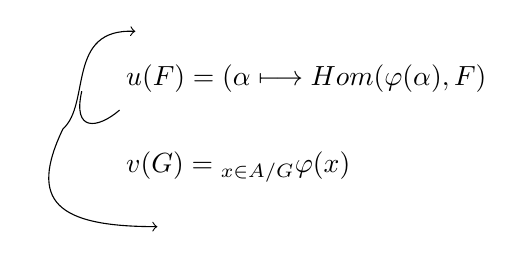
\begin{tikzpicture}[x=.8cm,y=.8cm]
\node[anchor=west] at (1.05,2.05) {$u(F)=(\alpha\longmapsto\operatorname{Hom}(\varphi(\alpha),F)$};
\node[anchor=west] at (1.05,.65) {$v(G)=\displaystyle\varinjlim_{x\in A/G}\varphi(x)$};
\draw[<->] (1.35,2.8) .. controls (.25,2.85) and (.65,1.65) .. (.2,1.25)
 .. controls (-.35,.1) and (.1,-.3) .. (1.7,-.3);
\draw (.5,1.85) .. controls (.35,1.2) and (.75,1.25) .. (1.1,1.55);
\end{tikzpicture}}

\par\noindent
\makebox[\linewidth][r]{%
  \smash{\begin{tabular}[t]{@{}l@{}}
  $u$ continu\\$v$ cocontinu
  \end{tabular}}%
}\par

\diagram{\begin{tikzcd}[ampersand replacement=\&,row sep=small,column sep=large]
\mathcal X\arrow[r]\&\widehat A\&\&\\
Y\&/\;a_i\to\varphi^*(Y)\&\varphi(a_i)\arrow[r]\&Y
\end{tikzcd}}

\end{minipage}
\end{lrbox}
\begin{center}
\begin{tikzpicture}
\node[anchor=south west,inner sep=0pt,outer sep=0pt] (spCancelledXVIII) at (0,0)
  {\usebox{\SPXCIIICancelledXVIII}};
% The unit vectors are the saved block's width and height.
\begin{scope}[x={(spCancelledXVIII.south east)},y={(spCancelledXVIII.north west)}]
% Descending course: upper left to lower right.
\draw[line width=.45pt] (.09,1.035)
 .. controls (.14,.96) and (.17,.84) .. (.26,.70)
 .. controls (.42,.49) and (.68,.15) .. (.81,.01);
% Opposing course, with the source's short upper pen gap.
\draw[line width=.45pt] (.50,1.00)
 .. controls (.50,.96) and (.44,.87) .. (.42,.835);
\draw[line width=.45pt] (.41,.812)
 .. controls (.36,.65) and (.21,.28) .. (.15,.13)
 .. controls (.145,.10) and (.14,.09) .. (.13,.08);
\end{scope}
\end{tikzpicture}
\end{center}
\endgroup

\margin{17}

\scanpage{19}
\mspage{\textcircled{2}}

\textbf{ACADEMIE D'AIX-MARSEILLE}\\
\rule{3cm}{.4pt}\\
\textbf{INSPECTION ACADEMIQUE}\\
\textbf{DE VAUCLUSE}\\
\rule{1cm}{.4pt}

\diagram{\begin{tikzcd}[ampersand replacement=\&,column sep=small,row sep=small]
I\arrow[r,"\text{épi}"]\arrow[dr,"\text{épi}"']\&J\arrow[r,no head]\arrow[dr,no head,bend right]\&{}\\
\&K.\&{}
\end{tikzcd}}
$\operatorname{card} I,J;K\leq3$

\diagram{\begin{tikzcd}[ampersand replacement=\&,column sep=small,row sep=small]
I\arrow[r]\arrow[d]\&J\arrow[r]\arrow[d]\&J'\arrow[d]\\
K\arrow[r]\&\deleted{\unsure{K'}}\arrow[r,no head]\&\bullet
\end{tikzcd}}

\diagram{\begin{tikzcd}[ampersand replacement=\&,column sep=small,row sep=small]
X_0\&X_1\arrow[l]\&X_2\arrow[l]\\
X'_0\arrow[u]\&X'_1\arrow[l]\arrow[u,no head,to path={(\tikztostart.north)--([yshift=-6pt]\tikztotarget.south)..controls([yshift=-2pt]\tikztotarget.south)and([xshift=-5pt,yshift=-2pt]\tikztotarget.south)..([xshift=-5pt,yshift=-5pt]\tikztotarget.south)\tikztonodes}]\&\unsure{X'_2|x'_2}\arrow[l]\arrow[u]
\end{tikzcd}}

\diagram{\begin{tikzcd}[ampersand replacement=\&,column sep=small,row sep=small]
I\arrow[r,hook]\arrow[d]\&J=I\amalg K\arrow[d,no head]\\
I'\arrow[r,hook,no head]\&J'=I'\amalg K
\end{tikzcd}}

\diagram{\begin{tikzcd}[ampersand replacement=\&,column sep=large,row sep=large]
X(I)\&\begin{gathered}\deleted{X(I)\times X(K)}\\
\inserted{X(I\amalg K)}\end{gathered}\arrow[l]\\
X(I')\arrow[u]\&X(I'\amalg K')\arrow[l]\arrow[u,no head,to path={
([yshift=2pt]\tikztostart.north) --
([yshift=-7pt]\tikztotarget.south)
.. controls ([xshift=3pt,yshift=-3pt]\tikztotarget.south)
and ([xshift=-3pt,yshift=-2pt]\tikztotarget.south)
.. ([xshift=-3pt,yshift=-5pt]\tikztotarget.south)\tikztonodes}]
\end{tikzcd}}

\diagram{\begin{tikzcd}[ampersand replacement=\&,column sep=large]
I\arrow[r]\&{}
\end{tikzcd}}

\diagram{\begin{tikzcd}[ampersand replacement=\&,column sep=large,row sep=large]
\mathbb E_n\arrow[r,"{\unsure{\delta|\partial}_n}"]\arrow[d,"K_{n-1}"]\&\mathbb E_{n+1}\\
\mathbb E_n\&{}
\end{tikzcd}}

\deleted{$\unsure{u}$}

\figure{\begin{tikzpicture}
\node at (0,0) {\begin{tikzcd}[ampersand replacement=\&,column sep=small,row sep=small]
\mathbb E_n\arrow[r,"{\unsure{\delta|\partial}_n}"]\arrow[d,"{\unsure{\delta|\partial}_n}"']\&\mathbb E_{n+1}\arrow[d]\\
\mathbb E_{n-1}\arrow[r]\&\mathbb E_{n+2}
\end{tikzcd}};
\node at (2.6,0) {$n\geq1$}; \node at (3.65,.8) {\textcircled{II}};
\node at (0,-2.6) {\begin{tikzcd}[ampersand replacement=\&,column sep=small,row sep=small]
\mathbb E_n\arrow[r,"{\unsure{\delta|\partial}_n}"]\arrow[d,"K_{n-1}"']\&\mathbb E_{n+1}\arrow[d]\\
\mathbb E_{n-1}\arrow[r,to path={(\tikztostart.east)--++(4pt,-2pt)--(\tikztostart.east)--(\tikztotarget.west)\tikztonodes}]\&\mathbb E_n
\end{tikzcd}};
\node at (2.6,-2.6) {$n\geq2$}; \node at (3.65,-2.7) {\textcircled{III}};
\draw (-2,-4)..controls(-1.6,-3.6)and(-1.4,-4.2)..(-1,-3.9)..controls(0,-4.2)and(1,-3.7)..(2,-4)..controls(2.5,-4.2)and(2.8,-3.8)..(3.2,-4);
\node at (0,-5.2) {\begin{tikzcd}[ampersand replacement=\&,column sep=small,row sep=small]
\mathbb E_{n\deleted{\unsure{*}}}\arrow[r,"K_{n-1}"]\arrow[d,"K'_{n-1}"']\&\mathbb E_{n-1}\arrow[d,no head,"{\deleted{\unsure{\alpha}}}"]\\
\mathbb E_{n-1}\arrow[r,no head,"{\deleted{\unsure{\alpha}}}",to path={(\tikztostart.east)--([xshift=-2pt]\tikztotarget.west)--++(0,3pt)\tikztonodes}]\&\mathbb E_{n-2}
\end{tikzcd}};
\node at (2.6,-5.2) {$n\geq3$}; \node at (3.65,-4.8) {\textcircled{IV}};
\node at (0,-7.8) {\begin{tikzcd}[ampersand replacement=\&,column sep=small,row sep=small]
\mathbb E_n\arrow[r,"K_{n-1}"]\arrow[d,"K''_{n-1}"']\&\mathbb E_{n-1}\arrow[d]\\
\mathbb E_{n-1}\arrow[r,no head,to path={(\tikztostart.east) -- ([xshift=-2pt]\tikztotarget.west) -- ++(-4pt,5pt)\tikztonodes}]\&\mathbb E_{n-2}
\end{tikzcd}};
\node at (2.6,-7.8) {$n\geq4$}; \node at (3.65,-7.7) {\textcircled{V}};
\draw (-2.2,.3)..controls(-2.7,2.2)and(2.4,2)..(3.5,.8)..controls(4.3,-1)and(4,-4)..(4.1,-6)..controls(4.4,-8)and(3.9,-9)..(2.8,-9.3);
\end{tikzpicture}}

\figure{\begin{tikzpicture}
\node at (0,0) {\begin{tikzcd}[ampersand replacement=\&,column sep=small,row sep=small]
\mathbb E_p\arrow[d]\&{}\\
\mathbb E_{p\unsure{+}q}\&\mathbb E_q\arrow[l]
\end{tikzcd}};
\node at (.3,1.4) {\textcircled{I}}; \node at (1.8,.6) {$p,q\geq1$};
\draw (-1.7,1.2)..controls(-.2,2)and(2.7,1.8)..(2.7,.2)..controls(2.7,-1.9)and(-.4,-2)..(-1.6,-.8)..controls(-2,-.5)and(-1.9,.2)..(-1.85,.55);
\end{tikzpicture}}

\figure{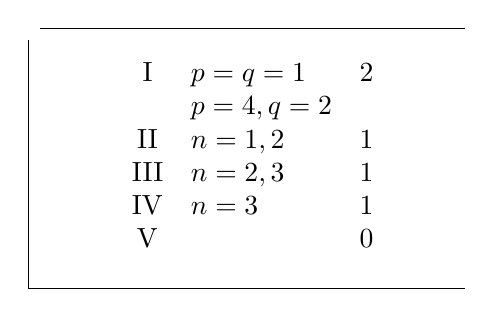
\begin{tikzpicture}
\node[inner sep=8pt] at (0,0) {$\begin{array}{clc}
\mathrm I&p=q=1&2\\
&p=4,q=2&\\
\mathrm {II}&n=1,\deleted{\unsure{2}}&1\\
\mathrm {III}&n=2,\deleted{\unsure{3}}&1\\
\mathrm {IV}&n=3&1\\
\mathrm V&&0
\end{array}$};
\draw (-2.7,1.65)--(2.7,1.65);
\draw (-2.85,1.5)--(-2.85,-1.65)--(2.7,-1.65);
\end{tikzpicture}}

\margin{$\deleted{\unsure{p|*}}$}

\figure{\begin{tikzpicture}[x=.012cm,y=-.012cm]
\node[anchor=west] at (835,1710) {$\mathrm I'$};
\node[anchor=west] at (925,1710) {$p=1,q=3$};
\node[anchor=west] at (925,1760) {$p=2,q=2$};
\node[anchor=west] at (835,1835) {$\mathrm {II}$};
\node[anchor=west] at (925,1835) {$n=2$};
\node[anchor=west] at (835,1902) {$\mathrm {III}$};
\node[anchor=west] at (925,1902) {$n=3$};
\node[anchor=west] at (835,1990) {$\mathrm {IV}$};
\node[anchor=west] at (925,1990) {$n=4$};
\node[anchor=west] at (835,2090) {$\mathrm V$};
\node[anchor=west] at (925,2090) {$n=4$};
\node at (1630,1678) {$2$};
\node at (1630,1810) {$1$};
\node at (1630,1891) {$1$};
\node at (1630,1985) {$1$};
\node at (1630,2080) {$1$};
\draw (810,1660)..controls(825,1800)and(812,2020)..(825,2220);
\draw (835,2180)..controls(1000,2190)and(1140,2145)..(1280,2150)
..controls(1420,2144)and(1530,2145)..(1570,2160);
\node at (1245,1655) {\begin{tikzcd}[ampersand replacement=\&,column sep=large]
\unsure{\mathbb E'}\arrow[r]\&\unsure{\mathbb E'}
\end{tikzcd}};
\node at (1260,1800) {\begin{tikzcd}[ampersand replacement=\&,column sep=large]
{}\arrow[r]\&{}
\end{tikzcd}};

\draw (1395,1795)--(1445,1795);
\draw (1395,1787)--(1395,1803);
\draw (1445,1787)--(1445,1803);
\node at (1465,1712) {$2$};
\node at (1220,1960) {\begin{tikzcd}[ampersand replacement=\&,column sep=small,row sep=large]
\mathbb E^2\&\mathbb E\arrow[l,no head]\\
\mathbb E^{\unsure{\prime|1}}\arrow[u,no head]\arrow[r,equals]\&
\mathbb E^{\unsure{\prime|1}}\arrow[u,no head,"{1}"']
\end{tikzcd}};
\node at (1470,1950) {\begin{tikzcd}[ampersand replacement=\&,column sep=small,row sep=large]
X^2\&X_{\unsure{1}}\arrow[l]\\
X_1\arrow[u]\arrow[r,equals]\&\unsure{X|x}_1\arrow[u,no head,"{1}"',to path={
([xshift=-3pt,yshift=2pt]\tikztostart.north)
.. controls ([xshift=2pt,yshift=1pt]\tikztostart.north)
and ([xshift=1pt,yshift=5pt]\tikztostart.north)
.. ([yshift=8pt]\tikztostart.north)
-- ([yshift=-7pt]\tikztotarget.south)
.. controls ([xshift=3pt,yshift=-3pt]\tikztotarget.south)
and ([xshift=-3pt,yshift=-2pt]\tikztotarget.south)
.. ([xshift=-3pt,yshift=-5pt]\tikztotarget.south)\tikztonodes}]
\end{tikzcd}};

\draw (1175,2143)--(1222,2143);
\draw (1175,2134)--(1175,2153);
\draw (1222,2134)--(1222,2153);
\draw (1286,2150)--(1286,2172);
\draw (1420,2139)--(1420,2168);
\draw (1468,2139)--(1468,2168);
% Cancellation strokes lie over the central diagrams, not over the table's live columns.
\draw[line width=.6pt] (1135,1600)
..controls(1110,1740)and(1090,1900)..(1120,2025)
..controls(1150,2110)and(1190,2110)..(1215,2110);
\draw[line width=.6pt] (1095,1855)--(1295,1600);
\draw[line width=.6pt] (1120,1785)
..controls(1190,1705)and(1245,1600)..(1260,1620)
..controls(1270,1650)and(1180,1835)..(1200,1800)
..controls(1300,1660)and(1395,1620)..(1370,1660);
\draw[line width=.6pt] (1115,2015)
..controls(1235,1860)and(1335,1720)..(1360,1745)
..controls(1380,1775)and(1240,1965)..(1260,1940)
..controls(1350,1840)and(1420,1810)..(1410,1875);
\draw[line width=.6pt] (1150,2080)
..controls(1220,2140)and(1250,1940)..(1290,1910)
..controls(1320,1890)and(1260,2080)..(1285,2070)
..controls(1340,1970)and(1430,1870)..(1420,1965);
\draw[line width=.6pt] (1350,1645)
..controls(1450,1540)and(1365,1790)..(1415,1760)
..controls(1520,1620)and(1475,1750)..(1510,1855);
\draw[line width=.6pt] (1505,1715)
..controls(1495,1870)and(1515,1910)..(1535,1750)
--(1580,2080)--(1495,2150);
\draw[line width=.6pt] (1400,2220)--(1550,1815);
\draw[line width=.6pt] (1230,2090)
..controls(1280,2050)and(1250,2160)..(1300,2145)
..controls(1370,2140)and(1380,2090)..(1420,2110);
\end{tikzpicture}}

\margin{18}

\scanpage{20}
\mspage{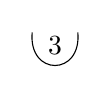
\begin{tikzpicture}[baseline=-.5ex]\node at (0,0) {3};\draw(-.29,.17)..controls(-.34,-.39)and(.34,-.39)..(.29,.17);\end{tikzpicture}}

\textbf{ACADEMIE D'AIX-MARSEILLE}\\
\rule{3cm}{.4pt}\\
\textbf{INSPECTION ACADEMIQUE}\\
\textbf{DE VAUCLUSE}\\
\rule{1cm}{.4pt}

\diagram{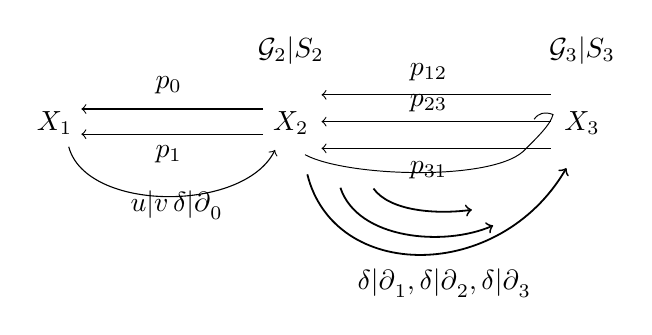
\begin{tikzpicture}[x=1cm,y=1cm]
\node at (0,0) {$X_1$}; \node at (3,0) {$X_2$}; \node at (6.7,0) {$X_3$};
\node at (3,.92) {$\unsure{\mathcal G_2|\mathfrak S_2}$};
\node at (6.7,.92) {$\unsure{\mathcal G_3|\mathfrak S_3}$};
\draw[->] (2.65,.18)--(.34,.18); \node at (1.45,.48) {$p_0$};
\draw[->] (2.65,-.14)--(.34,-.14); \node at (1.45,-.39) {$p_1$};
\draw[->] (.18,-.30)..controls(.40,-1.13)and(2.40,-1.14)..(2.80,-.34);
\node at (1.55,-1.04) {$\unsure{u|v}\,\unsure{\delta|\partial}_0$};
\draw[->] (6.30,.36)--(3.39,.36); \node at (4.75,.65) {$p_{12}$};
\draw[->] (6.30,.02)--(3.39,.02); \node at (4.75,.25) {$p_{23}$};
\draw[->] (6.30,-.32)--(3.39,-.32); \node at (4.75,-.60) {$p_{31}$};
\draw[line width=.35pt] (3.18,-.40)..controls(3.70,-.68)and(5.52,-.74)..(5.95,-.36)
 ..controls(6.12,-.19)and(6.30,-.02)..(6.33,.11)
 ..controls(6.22,.15)and(6.15,.13)..(6.09,.05);
\draw[->,line width=.65pt] (4.05,-.83)..controls(4.26,-1.12)and(4.85,-1.16)..(5.30,-1.10);
\draw[->,line width=.65pt] (3.63,-.82)..controls(3.85,-1.48)and(4.95,-1.57)..(5.57,-1.30);
\draw[->,line width=.65pt] (3.21,-.65)..controls(3.55,-2.02)and(5.65,-2.03)..(6.50,-.57);
\node at (4.95,-2.03) {$\unsure{\delta|\partial}_1,\unsure{\delta|\partial}_2,\unsure{\delta|\partial}_3$};
\end{tikzpicture}}
\margin{$\rho,\sigma_1,\sigma_2,\sigma_3$}

\deleted{$\unsure{p|\rho}=\unsure{q|\sigma}$}

\figure{\begin{tikzpicture}[x=1cm,y=1cm]
\node at (-1.8,.45) {$X_2$}; \node at (2.2,.45) {$X_1\times X_1$};
\node at (2.2,-1.10) {$X_1$};
\node at (-2.95,.45) {$\unsure{\mathcal G_2|\mathfrak S_2}$};
\draw[->] (-1.40,.45)--(1.44,.45); \draw(1.23,.57)--(1.40,.45)--(1.23,.33);
\node at (.10,.83) {$(p_0,p_1)\ \text{épi}$};
\node at (.16,1.50) {$p_0\sigma$}; \node at (.16,1.18) {$\Vert$};
\draw[->] (2.20,-.75)--(2.20,.10);
\draw(2.20,-.75)..controls(2.37,-.81)and(2.42,-.69)..(2.39,-.60);
\draw[->] (1.83,-.92)--(-1.45,.19);
\node at (.12,-.72) {$\unsure{\delta|\partial}_0$};
\draw(-2.23,1.70)--(2.55,1.85)..controls(2.95,1.83)and(2.96,1.76)..(2.96,1.33);
\draw(2.97,1.10)--(3.10,-.20)..controls(3.10,-.45)and(2.82,-.48)..(-2.10,-.40);
\draw(-2.23,-.30)--(-2.23,1.15);
\node at (-2.10,-2.52) {iso ???}; \draw(-2.10,-2.52) ellipse (1.05 and .49);
\draw[->] (-.32,.19)..controls(-.71,-.92)and(-3.26,-1.92)..(-2.91,-2.40);
\end{tikzpicture}}

\diagram{\begin{tikzpicture}[x=1cm,y=1cm]
\node at (0,0) {$X_3$}; \node at (3.55,0) {$X_2\times X_1$};
\node at (7.80,0) {$X_1\times X_1\times X_1$};
\draw[->] (.35,0)--(2.77,0); \draw(2.55,.12)--(2.72,0)--(2.55,-.12);
\node at (1.55,.35) {$(p_{12},q_3)\ \text{épi}$};
\draw[->] (4.32,0)--(6.48,0); \draw(6.25,.12)--(6.42,0)--(6.25,-.12);
\node at (5.43,.36) {$(p_0,p_1)\times\mathrm{id}_{X_1}$};
\draw[line width=.45pt] (-.27,.88)--(1.63,.83)..controls(2.25,.81)and(2.58,.53)..(3.04,.53)
 --(5.80,.53)..controls(5.96,.53)and(6.04,.58)..(6.06,.68);
\end{tikzpicture}}

\diagram{\begin{tikzpicture}[x=1cm,y=1cm]
\node at (0,0) {$X_3$};
\node at (3.72,0) {$\overset{(p_1)}{X_2}\times_{X_1}\overset{(p_0)}{X_2}$};
\node at (8.12,0) {$X_2\times_{X_1}(X_1\times X_1)$};
\draw[->] (.35,0)--(2.52,0); \draw(2.30,.12)--(2.47,0)--(2.30,-.12);
\node at (1.43,.34) {épi}; \node at (1.43,-.39) {$(p_{12},p_{23})$};
\draw[->] (4.93,0)--(6.22,0); \draw(6.00,.12)--(6.17,0)--(6.00,-.12);
\node at (5.58,.35) {épi};
\draw(-.47,.66)--(4.99,.73);
\draw(5.12,.60)--(5.15,-.54);
\draw(4.99,-.67)--(-.43,-.63);
\draw(-.55,-.51)--(-.57,.55);
\end{tikzpicture}}

\diagram{\begin{tikzcd}[ampersand replacement=\&]
\mathbb E_1\arrow[r]\arrow[d,no head,to path={([xshift=3pt,yshift=-4pt]\tikztostart.south)--(\tikztostart.south)--(\tikztotarget.north)--++(-3pt,4pt)\tikztonodes}]\&\mathbb E_2\arrow[d]\\
\mathbb E_2\arrow[r]\&\mathbb E_3
\end{tikzcd}}

\figure{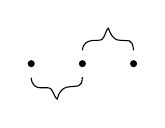
\begin{tikzpicture}[x=1cm,y=1cm]
\fill(0,0)circle(.045); \fill(.65,0)circle(.045); \fill(1.30,0)circle(.045);
\draw(0,-.18)..controls(.02,-.38)and(.20,-.27)..(.25,-.32)
 ..controls(.28,-.35)and(.30,-.44)..(.33,-.45)
 ..controls(.35,-.36)and(.40,-.31)..(.45,-.30)
 ..controls(.60,-.27)and(.64,-.32)..(.65,-.17);
\draw(.65,.17)..controls(.67,.35)and(.86,.27)..(.90,.31)
 ..controls(.94,.34)and(.95,.44)..(.98,.45)
 ..controls(1.01,.36)and(1.05,.31)..(1.10,.30)
 ..controls(1.25,.28)and(1.28,.33)..(1.30,.17);
\end{tikzpicture}}

\diagram{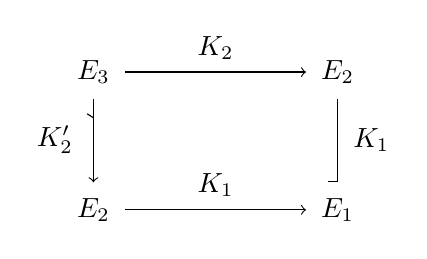
\begin{tikzpicture}[x=1cm,y=1cm]
\node at (0,0) {$\mathbb E_3$}; \node at (3.1,0) {$\mathbb E_2$};
\node at (0,-1.75) {$\mathbb E_2$}; \node at (3.1,-1.75) {$\mathbb E_1$};
\draw[->] (.40,0)--(2.70,0); \node at (1.55,.30) {$K_2$};
\draw[->] (0,-.34)--(0,-1.40); \draw(0,-.58)--(-.08,-.53);
\node at (-.49,-.86) {$K'_2$};
\draw(3.10,-.34)--(3.10,-1.39)--(2.98,-1.39);
\node at (3.53,-.86) {$K_1$};
\draw[->] (.40,-1.75)--(2.70,-1.75); \node at (1.55,-1.43) {$K_1$};
\end{tikzpicture}}

\figure{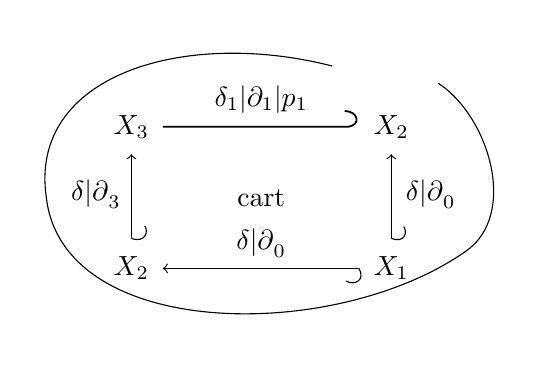
\begin{tikzpicture}[x=1cm,y=1cm]
\node at (0,0) {$X_3$}; \node at (3.3,0) {$X_2$};
\node at (0,-1.80) {$X_{\unsure{2}}$}; \node at (3.3,-1.80) {$X_1$};
\draw[line width=.65pt] (.40,0)--(2.76,0)..controls(2.91,.02)and(2.89,.19)..(2.71,.20);
\node at (1.65,.34) {$\unsure{\delta_1|\partial_1|p_1}$};
\draw[->] (0,-1.42)--(0,-.35);
\draw(0,-1.42)..controls(.18,-1.48)and(.22,-1.33)..(.17,-1.26);
\node at (-.45,-.86) {$\unsure{\delta|\partial}_3$};
\draw[->] (3.30,-1.42)--(3.30,-.35);
\draw(3.30,-1.42)..controls(3.47,-1.48)and(3.51,-1.35)..(3.46,-1.27);
\node at (3.80,-.86) {$\unsure{\delta|\partial}_0$};
\draw[->] (2.89,-1.80)--(.40,-1.80);
\draw(2.89,-1.80)..controls(2.98,-1.96)and(2.82,-2.02)..(2.73,-1.96);
\node at (1.65,-1.48) {$\unsure{\delta|\partial}_0$};
\node at (1.65,-.91) {cart};
\draw(2.55,.77)..controls(.68,1.25)and(-1.31,.66)..(-1.08,-.90)
 ..controls(-.87,-2.72)and(2.59,-2.75)..(4.25,-1.58)
 ..controls(4.91,-1.12)and(4.55,.12)..(3.90,.55);
\end{tikzpicture}}

\diagram{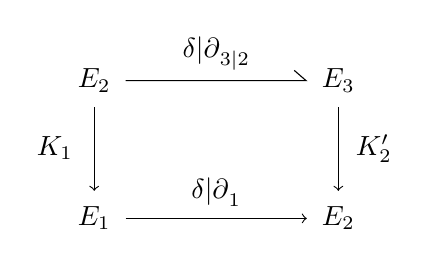
\begin{tikzpicture}[x=1cm,y=1cm]
\node at (0,0) {$\mathbb E_2$}; \node at (3.1,0) {$\mathbb E_3$};
\node at (0,-1.75) {$\mathbb E_1$}; \node at (3.1,-1.75) {$\mathbb E_2$};
\draw(.40,0)--(2.69,0)--(2.54,.13);
\node at (1.55,.34) {$\unsure{\delta|\partial}_{\unsure{3|2}}$};
\draw[->] (0,-.34)--(0,-1.40); \node at (-.50,-.86) {$K_{\unsure{1}}$};
\draw[->] (3.10,-.34)--(3.10,-1.40); \node at (3.55,-.86) {$K'_2$};
\draw[->] (.40,-1.75)--(2.70,-1.75);
\node at (1.55,-1.42) {$\unsure{\delta|\partial}_1$};
\end{tikzpicture}}

\figure{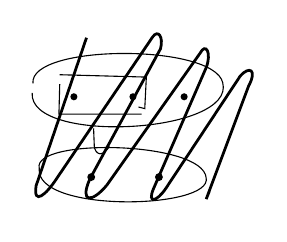
\begin{tikzpicture}[x=1cm,y=1cm]
\draw(-1.17,.17)..controls(-1.22,.67)and(1.12,.68)..(1.24,.18)
 ..controls(1.41,-.47)and(-1.23,-.61)..(-1.18,.05);
\draw(-.83,.28)--(.27,.25)--(.25,-.15)--(.17,-.13);\draw(.21,-.22)--(-.84,-.22)--(-.83,.16);
\fill(-.65,0)circle(.045); \fill(.10,0)circle(.045); \fill(.75,0)circle(.045);
\draw(-1.09,-.91)..controls(-1.19,-.52)and(.99,-.56)..(1.03,-1.03)
 ..controls(1.11,-1.43)and(-1.15,-1.48)..(-1.09,-.91);
\fill(-.43,-1.02)circle(.05); \fill(.43,-1.02)circle(.05);
\draw(-.40,-.40)--(-.39,-.65)..controls(-.34,-.79)and(-.24,-.70)..(-.20,-.63);
\draw[line width=1pt] (-.49,.75)--(-1.13,-1.13)
 ..controls(-1.17,-1.39)and(-1.00,-1.24)..(-.87,-1.04)
 --(.35,.76)..controls(.42,.86)and(.49,.76)..(.45,.61)
 --(-.45,-1.05)..controls(-.58,-1.35)and(-.42,-1.35)..(-.23,-1.12)
 --(.95,.55)..controls(1.03,.70)and(1.10,.55)..(1.03,.37)
 --(.36,-1.17)..controls(.28,-1.36)and(.40,-1.34)..(.52,-1.16)
--(1.46,.26)..controls(1.58,.40)and(1.68,.34)..(1.57,.14)--(1.03,-1.30)--(1.07,-1.20);
\end{tikzpicture}}

\figure{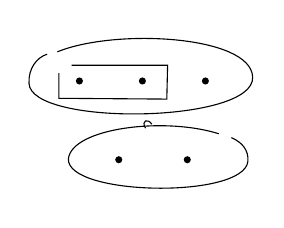
\begin{tikzpicture}[x=1cm,y=1cm]
\draw(-.93,.37)..controls(-.20,.67)and(1.53,.58)..(1.55,.05)
 ..controls(1.58,-.54)and(-1.27,-.58)..(-1.29,-.03)
 ..controls(-1.30,.16)and(-1.19,.30)..(-1.06,.34);
\draw(-.75,.20)--(.47,.20)--(.46,-.23)--(-.91,-.22)--(-.91,.10);
\fill(-.65,0)circle(.045); \fill(.15,0)circle(.045); \fill(.95,0)circle(.045);
\draw(1.12,-.67)..controls(.42,-.45)and(-.75,-.60)..(-.79,-.99)
 ..controls(-.81,-1.46)and(1.44,-1.50)..(1.49,-1.02)
 ..controls(1.50,-.88)and(1.42,-.78)..(1.28,-.72);
\draw(.19,-.60)..controls(.13,-.50)and(.22,-.47)..(.27,-.55);
\fill(-.15,-1.00)circle(.045); \fill(.72,-1.00)circle(.045);
\end{tikzpicture}}

\figure{\unsure{\mbox{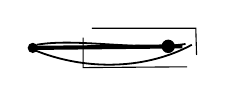
\begin{tikzpicture}[x=1cm,y=1cm]
\draw[line width=1.5pt] (-.80,0)--(1.12,.02);
\fill(-.78,0)circle(.065); \fill(.94,.02)circle(.085);
\draw(-.03,.25)--(1.29,.25)--(1.30,-.09);
\draw(1.18,-.24)--(-.14,-.25)--(-.14,.13);
\draw[line width=.65pt] (-.78,-.02)..controls(-.08,-.31)and(.69,-.26)..(1.24,.04);
\draw[line width=.65pt] (-.73,.04)..controls(-.22,.13)and(.57,-.04)..(1.16,.05);
\end{tikzpicture}}}}

\figure{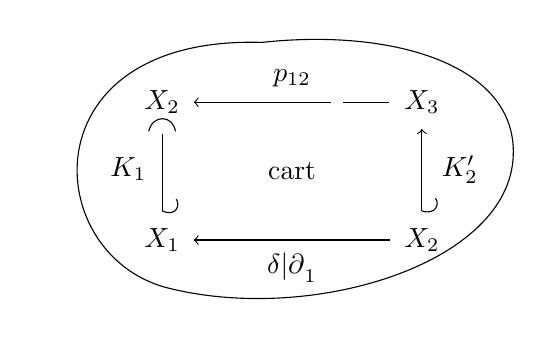
\begin{tikzpicture}[x=1cm,y=1cm]
\node at (0,0) {$X_2$}; \node at (3.3,0) {$X_3$};
\node at (0,-1.75) {$X_1$}; \node at (3.3,-1.75) {$X_2$};
\draw[<-] (.40,0)--(2.15,0); \draw(2.30,0)--(2.88,0);
\node at (1.65,.31) {$p_{12}$};
\draw(0,-1.38)--(0,-.40);\draw(-.17,-.37)..controls(-.12,-.15)and(.14,-.16)..(.17,-.37);
\draw(0,-1.38)..controls(.19,-1.46)and(.23,-1.30)..(.18,-1.23);
\node at (-.43,-.85) {$K_1$};
\draw[->] (3.30,-1.38)--(3.30,-.34);
\draw(3.30,-1.38)..controls(3.48,-1.44)and(3.53,-1.28)..(3.47,-1.22);
\node at (3.78,-.85) {$K'_2$};
\draw[->] (2.89,-1.75)--(.40,-1.75);
\node at (1.65,-2.10) {$\unsure{\delta|\partial}_1$};
\node at (1.65,-.87) {cart};
\draw(1.27,.76)..controls(-1.70,.85)and(-1.55,-1.91)..(.04,-2.35)
 ..controls(1.87,-2.83)and(4.42,-2.06)..(4.46,-.67)
 ..controls(4.50,.49)and(2.90,.94)..(1.27,.76);
\end{tikzpicture}}

\diagram{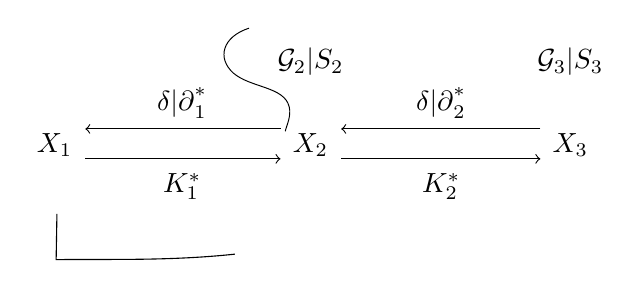
\begin{tikzpicture}[x=1cm,y=1cm]
\node at (0,0) {$X_1$}; \node at (3.25,0) {$X_2$}; \node at (6.55,0) {$X_3$};
\node at (3.25,1.05) {$\unsure{\mathcal G_2|\mathfrak S_2}$};
\node at (6.55,1.05) {$\unsure{\mathcal G_3|\mathfrak S_3}$};
\draw[->] (2.87,.20)--(.39,.20);
\node at (1.62,.53) {${\unsure{\delta|\partial}}_1^*$};
\draw[->] (.39,-.18)--(2.87,-.18); \node at (1.62,-.53) {$K_{\unsure{1}}^*$};
\draw[->] (6.17,.20)--(3.64,.20);
\node at (4.91,.53) {${\unsure{\delta|\partial}}_2^*$};
\draw[->] (3.64,-.18)--(6.17,-.18); \node at (4.91,-.53) {$K_2^*$};
\draw[line width=.35pt] (2.47,1.48)..controls(2.13,1.37)and(2.06,1.10)..(2.27,.91)
 ..controls(2.49,.72)and(2.92,.74)..(2.98,.48)
 ..controls(3.01,.36)and(2.94,.23)..(2.93,.17);
\draw(.03,-.88)--(.02,-1.46)..controls(.65,-1.45)and(1.45,-1.48)..(2.29,-1.39);
\end{tikzpicture}}

\deleted{$\unsure{\mathbb E}$}

\noindent Supposons $X_1$ réduit\\
à un élément, donc\\
$X_2$ est un $\unsure{\mathcal G_2|\mathfrak S_2}$-ens. à pt\\
fixe marqué $\unsure{\delta|\partial}_2$, $X_3$ un\\
$\unsure{\mathcal G_3|\mathfrak S_3}$-ens. à pt fixe marqué $\unsure{\delta|\partial}_3$

\diagram{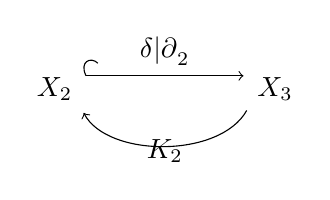
\begin{tikzpicture}[x=1cm,y=1cm]
\node at (0,0) {$X_2$}; \node at (2.8,0) {$X_3$};
\draw[->] (.40,.17)--(2.40,.17);
\draw(.40,.17)..controls(.31,.35)and(.46,.42)..(.55,.33);
\node at (1.40,.48) {$\unsure{\delta|\partial}_2$};
\draw[->] (2.44,-.27)..controls(2.10,-.88)and(.67,-.87)..(.37,-.30);
\node at (1.40,-.78) {$K_2$};
\end{tikzpicture}}

\deleted{$\unsure{\delta|\partial}_{\unsure{2}}$} $\unsure{\delta|\partial}_2$ et $K_2$\\
compatibles avec\\
les \deleted{\unsure{pts fixes}} \inserted{\unsure{ponctuations|pointations|structures}}\\
par $\unsure{\delta|\partial}_2,\unsure{\delta|\partial}_3$, avec
\[
K_2\unsure{\delta|\partial}_2=\mathrm{id}_{X_2}
\]

\diagram{\begin{tikzcd}[ampersand replacement=\&]
\mathbb E_1\arrow[r,hook]\&\mathbb E_2\arrow[l,bend left=45]
\end{tikzcd}}

\figure{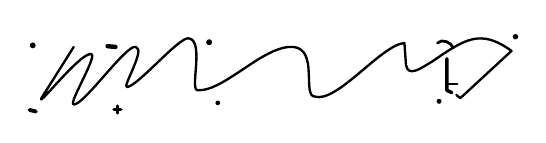
\begin{tikzpicture}[x=1cm,y=1cm,line cap=round,line join=round]
\draw[line width=.85pt] (.57,.75)--(.16,.10)
 ..controls(.10,-.03)and(.63,.65)..(.78,.66)
 ..controls(.91,.69)and(.49,.02)..(.57,.02)
 ..controls(.69,.00)and(1.25,.80)..(1.36,.75)
 ..controls(1.49,.72)and(1.17,.22)..(1.25,.24)
 ..controls(1.40,.27)and(1.91,.88)..(2.03,.86)
 ..controls(2.24,.83)and(2.03,.18)..(2.15,.20)
 ..controls(2.49,.19)and(2.99,.78)..(3.36,.75)
 ..controls(3.68,.72)and(3.47,.13)..(3.63,.12)
 ..controls(3.91,.03)and(4.48,.78)..(4.77,.80)
 --(4.79,.52)..controls(4.82,.36)and(4.98,.48)..(5.13,.57)
 ..controls(5.55,.86)and(5.74,.98)..(6.13,.70)
 --(5.48,.10)--(5.43,.14);
\fill(.05,.77)circle(.037); \draw[line width=1.4pt] (.01,-.05)--(.09,-.07);
\draw[line width=1.6pt] (1.00,.76)--(1.10,.75);
\draw[line width=1.15pt] (1.13,.00)--(1.13,-.09); \draw[line width=1.15pt] (1.08,-.04)--(1.17,-.04);
\fill(2.29,.81)circle(.038); \fill(2.40,.04)circle(.030);
\draw[line width=1pt] (5.19,.80)..controls(5.25,.86)and(5.36,.81)..(5.39,.74);
\fill(6.18,.88)circle(.035); \fill(5.21,.06)circle(.032);
\draw[line width=1.3pt] (5.31,.60)--(5.31,.20)--(5.37,.17);
\draw[line width=.9pt] (5.30,.28)--(5.44,.28);
\end{tikzpicture}}

\margin{19}

\scanpage{21}

\[
\unsure{\zeta|\xi}=(\unsure{x},y)\qquad d\sigma(\unsure{\zeta|\xi})=(y,x,\unsure{x|n})
\]
\[
\rho^2d(\unsure{\zeta|\xi})=(y,x,y)
\]

\margin{20}

\scanpage{22}
\mspage{\textcircled{4}}

\textbf{\textsf{ACADEMIE D'AIX-MARSEILLE}}\\
\rule{3cm}{.4pt}\\
\textbf{INSPECTION ACADEMIQUE}\\
\textbf{DE VAUCLUSE}\\
\rule{1cm}{.4pt}

\deleted{$\unsure{\mathcal G|\mathfrak S}$}
\[
\unsure{\mathcal G_2|\mathfrak S_2}=\{1,\sigma\}\qquad
\unsure{\mathcal G_3|\mathfrak S_3}=\{1,\rho,\rho^2,\sigma_1,\sigma_2,\sigma_3)
\]
\margin{$[\rho^3=1,\inserted{\sigma_i^2=1,}\rho\sigma_i\rho^{-1}=\sigma_{i+1}\quad(\sigma_4=\sigma_1)]$}

\diagram{\begin{tikzcd}[ampersand replacement=\&,row sep=small,column sep=large]
X_1\arrow[d,phantom,"\Vert"]\&X_2\arrow[d,phantom,"\in" rotate=90]\arrow[r,shift left,"d"]\&X_3\arrow[l,shift left,"p"]\arrow[d,phantom,"\in" rotate=90]\\
\{e_1\}\&e_2\&e_3
\end{tikzcd}}
\[
\sigma e_2=e_2
\]
\margin{$-$}

\[
d(x,y)=(x,y,y)\qquad\rho d(x,y)=(y,y,x)\qquad\rho^2d(x,y)=(y,x,y)
\]
\[
p(x,y,z)=(x,y)
\]
\[
\begin{aligned}
\rho(x,y,z)&=(y,z,x)\\
\rho^2(x,y,z)&=(z,x,y\unsure{]|)}\\
\sigma_1(x,y,z)&=(x,z,y)\\
\sigma_2(x,y,z)&=(z,y,x)\\
\sigma_3(x,y,z)&=(y,x,z)
\end{aligned}
\]
\figure{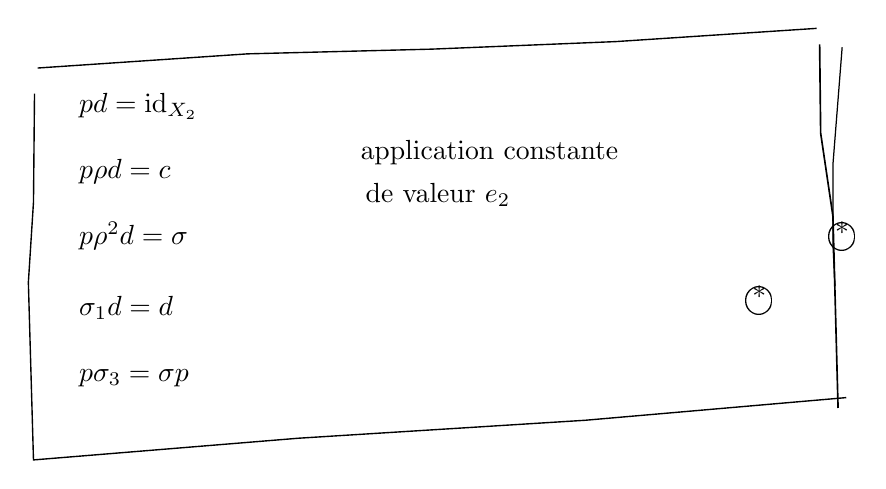
\begin{tikzpicture}[x=.013cm,y=.012cm,every node/.style={inner sep=0pt}]
\node[anchor=base west] at (65,-95) {$pd=\mathrm{id}_{X_2}$};
\node[anchor=base west] at (65,-165) {$p\rho d=c$};
\node[anchor=base west] at (340,-145) {application constante};
\node[anchor=base west] at (345,-190) {de valeur $e_2$};
\node[anchor=base west] at (65,-235) {$p\rho^2d=\sigma$};
\node[anchor=base west] at (65,-310) {$\sigma_1d=d$};
\node[anchor=base west] at (65,-380) {$p\sigma_3=\sigma p$};
\node[anchor=center] at (730,-294) {\textcircled{*}};
\node[anchor=center] at (811,-226) {\unsure{\textcircled{*}}};
\draw[line width=.5pt] (25,-48) -- (230,-33) -- (410,-28) -- (590,-20) -- (786,-6);
\draw[line width=.5pt] (22,-75) -- (21,-190) -- (16,-275) -- (21,-463) -- (280,-440) -- (560,-421) -- (815,-397);
\draw[line width=.6pt] (789,-23) -- (790,-117) -- (802,-205) -- (807,-408);
\draw[line width=.45pt] (811,-26) -- (802,-150) -- (802,-235) -- (804,-279);
\end{tikzpicture}}

\[
\unsure{\mathcal G_3|\mathfrak S_3}
=\deleted{\unsure{\{1,\rho,\rho^2\}}}\{1,\sigma_1\}\cdot\{1,\rho,\rho^2\}
=\underbrace{\{1,\rho,\rho^2\}}_{\substack{\unsure{\rotatebox{90}{$\in$}}\\g}}\cdot\underbrace{\{1,\sigma_1\}}_{\substack{\rotatebox{90}{$\in$}\\h}}
\]
\[
d(X_2)\subset X_3\qquad(g\circ h)\circ d=g\circ d
\]
\[
\begin{gathered}
[\rho^i d(\unsure{\zeta|\xi}\deleted{\unsure{'}})=\rho^{i'}d(\unsure{\zeta'|\xi'})]
\ \substack{\overset{?}{\Longrightarrow}\\[-2pt]\Longleftarrow}\
[i\equiv i'\ (3),\ \unsure{\zeta|\xi}=\unsure{\zeta'|\xi'}]\\
\Updownarrow\\
[d(\unsure{\zeta'|\xi'})=\rho^{i\deleted{\unsure{'}}-i'}d(\unsure{\zeta|\xi}\deleted{\unsure{'}})]
\end{gathered}
\]
\margin{\inserted{ou $[\unsure{\zeta|\xi}=\unsure{\zeta'|\xi'}=e_2]$}}

\[
d(\unsure{\zeta'|\xi'})=\rho^j d(\unsure{\zeta|\xi}\deleted{\unsure{'}})
\left\{\begin{aligned}
&\text{si }j=0\quad\text{on a}\quad\unsure{\zeta'|\xi'}=\unsure{\zeta|\xi}\quad\text{cqfd}\\
&\text{si }j=1\quad\text{on a}\quad\unsure{\zeta'|\xi'}=p\rho d(\unsure{\zeta|\xi})=e_2\\
&\text{donc}\quad\underset{\substack{\Vert\\\inserted{d(\unsure{\zeta'|\xi'})=d(e_2)}}}{e_3}=\rho d(\unsure{\zeta|\xi})\\
&\text{donc}\quad d(\unsure{\zeta|\xi})=e_3\quad\text{donc}\\
&\deleted{\text{donc}\quad d(\unsure{\zeta|\xi})=e_3}\\
&\unsure{\zeta|\xi}=pd(\unsure{\zeta|\xi})=pe_3=e_2\\
&\text{donc}\quad\unsure{\zeta|\xi}\deleted{\unsure{'}}=\unsure{\zeta'|\xi'}=e_2\\
&\text{si }j=2,\quad\unsure{\zeta'|\xi'}=p\rho^2d(\unsure{\zeta|\xi})=\sigma\unsure{\zeta|\xi}
\end{aligned}\right.
\]
\margin{$d\sigma(\unsure{\zeta|\xi})=\rho^2d(\unsure{\zeta|\xi})\qquad d(\unsure{\zeta|\xi})=\rho d\sigma(\unsure{\zeta|\xi})$
\[
\unsure{\zeta|\xi}=p\rho d\sigma(\unsure{\zeta|\xi}\unsure{]|)}=e_2,\quad\unsure{\zeta'|\xi'}=e_2
\]}

\margin{21}

\scanpage{23}
\mspage{5}

Ainsi, le sous-$\unsure{\mathcal G_3|\mathfrak S_3}$-ens. \inserted{$X'_3$} de $X_3$ engendré par $d(X_2)$ a une unique orbite à 1 \unsure{élémt}, savoir $\{e_3\}=\{de_2\}$, toutes les autres orbites sont de cardinal 3 \deleted{et} (dans la représentation régulière de $\unsure{\mathcal G_3|\mathfrak S_3|\deleted{\mathcal G}_3|\deleted{\mathfrak S}_3}$), et elles sont en corr. biunivoque avec les éléments de $X_2\setminus\{e_2\}\overset{\mathrm{def}}=X_2^*$. Comme $\unsure{\mathcal G_3|\mathfrak S_3}$-ens $X'_3$ s'écrit canoniquement
% The two X-shaped overstrokes are retained locally as live/struck alternatives; their function is unresolved.
\[
X'_3\simeq\{e_3\}\amalg\left(\unsure{\mathcal G_3|\mathfrak S_3|\deleted{\mathcal G}_3|\deleted{\mathfrak S}_3}\wedge_{\{1,\sigma_1\}}X_2^*\right),
\]
où $\{1,\sigma_1\}$ opère trivialement sur $X_2^*$

\margin{Et on a une explicitation de $p$ sur $X'_3$ via les trois premières des cinq formules $(*)$, \unsure{le reste} à satisfaire \unsure{étant} \unsure{formel} \unsure{par ces trois formules} \unsure{cas|(a)}}

Reste à exprimer
\[
X_3^*\overset{\mathrm{def}}=X_3\setminus\underbrace{X'_3}_{\unsure{\mathcal G_3|\mathfrak S_3}\cdot d(X_2)}
\]
comme $\unsure{\mathcal G_3|\mathfrak S_3}$-ens, et l'application induite par $p$
% One shaft with two separated complete rightward heads.
\diagram{\begin{tikzcd}[ampersand replacement=\&,column sep=large]
X_3^*\arrow[r,"p^*=p\mid X_3^*"]\arrow[r,shorten >=12pt]\&X_2
\end{tikzcd}}
satisfaisant à
\figure{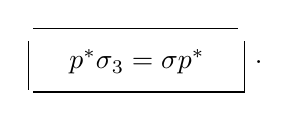
\begin{tikzpicture}[baseline=(rel.base)]
\node[inner sep=4pt] (rel) at (0,0) {$p^*\sigma_3=\sigma p^*$};
\draw[line width=.45pt] (-1.32,.43)--(1.28,.43);
\draw[line width=.45pt] (-1.38,.27)--(-1.38,-.36);
\draw[line width=.45pt] (-1.32,-.38)--(1.37,-.38)--(1.37,.27);
\node[anchor=west,inner sep=0pt] at (1.49,0) {.};
\end{tikzpicture}}

\diagram{\begin{tikzcd}[ampersand replacement=\&,column sep=large]
X_3\arrow[r,two heads,"{p,p\rho}"]\&X_2\times X_2\&\text{épi}
\end{tikzcd}}

\margin{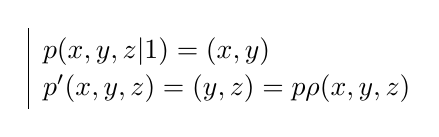
\begin{tikzpicture}[baseline=(r1.base)]
\draw[line width=.45pt] (0,.30)--(0,-.72);
\node[anchor=west,inner sep=0pt] (r1) at (.18,0) {$p(x,y,\unsure{z|1})=(x,y)$};
\node[anchor=west,inner sep=0pt] at (.18,-.47) {$p'(x,y,z)=(y,z)=p\rho(x,y,z)$};
\end{tikzpicture}}

pour $\unsure{\zeta|\xi},\eta\in X_2$, $\exists\alpha\in X_3$ avec
\[
p\alpha=\unsure{\zeta|\xi},\quad p\rho\alpha=\eta
\]

\margin{22}

\scanpage{24}
\mspage{\textcircled{6}}

\textsf{\textbf{ACADEMIE D'AIX-MARSEILLE}}\\
\rule{3cm}{.4pt}\\
\textbf{INSPECTION ACADEMIQUE}\\
\textbf{DE VAUCLUSE}\\
\rule{1cm}{.4pt}

Quelle est la partie de $X_2\times X_2$ qui provient de $X'_3$ ?

\[
\text{a)}\quad(p,p\rho)(e_3)=(e_2,e_2)
\]
\[
\text{b)}\quad(p,p\rho)
\underset{\substack{i\in\mathbb Z/3\mathbb Z\\\unsure{\xi|\zeta}\in X_2^*=X_2\setminus\{e_2\}}}{
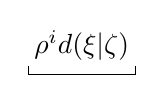
\begin{tikzpicture}[baseline=(term.base)]
\node[inner sep=1pt] (term) {$\rho^i d(\unsure{\xi|\zeta})$};
\draw[line width=.45pt] ([xshift=-1pt,yshift=-1pt]term.south west) -- ([xshift=-1pt,yshift=-4pt]term.south west) -- ([xshift=1pt,yshift=-4pt]term.south east) -- ([xshift=1pt,yshift=-1pt]term.south east);
\end{tikzpicture}}
=\begin{cases}
(\unsure{\xi|\zeta},e_2)&\text{si }i=0\\
(e_2,\sigma\unsure{\xi|\zeta})&\text{si }i=1\\
(\sigma\unsure{\xi|\zeta},\unsure{\xi|\zeta})&\text{si }i=2
\end{cases}
\]

Donc on trouve les éléments \deleted{de la \unsure{forme}} dans
\[
\uline{\underbrace{(X_2\times\{e_2\})}_{\Sigma_1}\cup\underbrace{(\{e_2\}\times X_2)}_{\Sigma_2}\cup\deleted{\unsure{\Delta}}\Delta'}
\]
où $\Delta'$ est l'image de
\figure{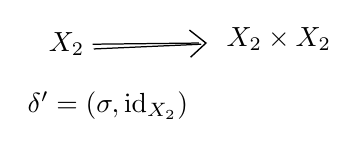
\begin{tikzpicture}[x=.015cm,y=.015cm,every node/.style={inner sep=0pt}]
\node[anchor=base] at (0,0) {$X_2$};
\node[anchor=base west] at (135,4) {$X_2\times X_2$};
\node[anchor=base] at (35,-52) {$\delta'=(\sigma,\mathrm{id}_{X_2})$};
\draw[line width=.45pt] (22,6) -- (112,7);
\draw[line width=.45pt] (23,2) -- (114,6);
\draw[line width=.5pt] (104,18) -- (118,7) -- (105,-5);
\end{tikzpicture}}

\uline{NB} Cette partie $\Sigma$ de $X_2\times X_2$ est la réunion de $\Sigma_{\unsure{1|0}},\Sigma_2,\Delta'$, dont l'intersection de deux parmi les trois est égale à $\{(e_2,e_2)\}$

Quand a-t-on $\Sigma=X_2\times X_2$ ?

\deleted{\unsure{Si}} On a
\[
X_2\times X_2\longrightarrow\{\Sigma_1\cup\Sigma_2)=X_2^*\times X_2^*,
\]
donc il est n et s. que $X_2^*\longrightarrow X_2^*\times X_2^*$ soit surj., i.e. que pour $\unsure{\zeta|\xi},\eta\in X_2^*$, on ait tjs $\eta=\sigma\unsure{\zeta|\xi}$. Cela signifie que l'on est dans l'un des 2 cas suivants

a) $X_2^*=\unsure{\phi|\varnothing}$ i.e. $X_2=\{e_2\}$

b) $X_2^*$ de cardinal 1 (donc $\sigma$ \deleted{\unsure{y}} y opère \unsure{trivialt})

\reversemarginpar
\margin{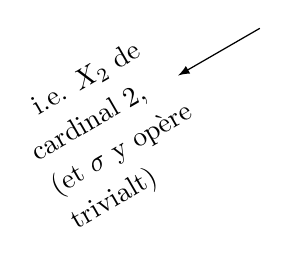
\begin{tikzpicture}[rotate=30,transform shape,every node/.style={inner sep=0pt}]
\node[anchor=base west] at (0,0) {i.e. $X_2$ de};
\node[anchor=base west] at (-.3,-.5) {cardinal $2$,};
\node[anchor=base west] at (-.3,-1) {(et $\sigma$ y opère};
\node[anchor=base west] at (-.3,-1.5) {\unsure{trivialt})};
\draw[-latex,line width=.45pt] (3,-.45) -- (1.8,-.45);
\end{tikzpicture}}
\normalmarginpar

[Si $X_2^*$ est de cardinal $\geq2$, alors s'il y a une seule orbite sous $\sigma$, celle-ci est de cardinal 2, et \deleted{$\unsure{\xi}$} $\forall\unsure{\zeta|\xi}\in X_2^*)$ $(\unsure{\zeta|\xi},\unsure{\zeta|\xi})\notin\operatorname{Im}\delta'$ i.e. $\unsure{\zeta|\xi}\ne\sigma\unsure{\zeta|\xi}$). ou s'il y a \deleted{\unsure{deux|donc}} au moins deux orbites, on prend $\unsure{\zeta|\xi},\eta$ dans deux orbites différentes, et on a bien $\eta\ne\sigma\unsure{\zeta|\xi}$.

\margin{23}

\scanpage{25}

\mspage{\textcircled{7}}

\margin{$X_2=\{e_2,\unsure{\zeta|\xi})$}
Supposons \inserted{donc} $X_2$ de cardinal 2, \deleted{\unsure{donc}} et \deleted{\unsure{que}} $X_3=X'_3$ donc
\[
X_3=\{e_3\}\amalg\{d\unsure{\zeta|\xi},\rho d\unsure{\zeta|\xi},\rho^2d\unsure{\zeta|\xi}\},
\]
considérons les deux carrés

\diagram{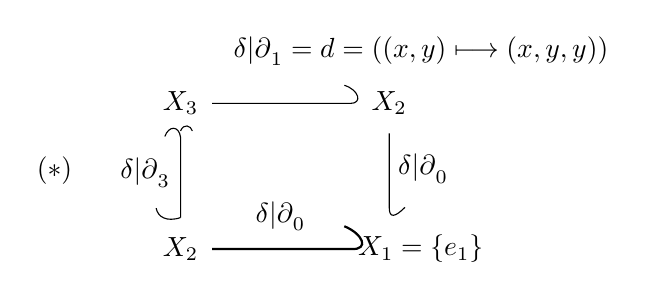
\begin{tikzpicture}[x=1cm,y=1cm]
\node at (-1.60,-.85) {$(*)$};
\node at (0,0) {$X_3$}; \node at (2.65,0) {$X_2$};
\node at (0,-1.85) {$X_2$}; \node at (3.05,-1.85) {$X_1=\{e_1\}$};
\draw(.40,0)--(2.16,0)..controls(2.31,.00)and(2.27,.17)..(2.08,.23);
\node[anchor=west] at (.55,.66) {$\unsure{\delta|\partial}_1=d=((x,y)\longmapsto(x,y,y))$};
\draw(0,-1.45)--(0,-.43)..controls(-.02,-.28)and(-.15,-.28)..(-.20,-.42);
\draw(0,-.35)..controls(.04,-.25)and(.13,-.28)..(.15,-.35);
\draw(0,-1.45)..controls(-.18,-1.51)and(-.29,-1.44)..(-.31,-1.33);
\node at (-.45,-.88) {$\unsure{\delta|\partial}_3$};
\draw(2.65,-.38)--(2.65,-1.32)..controls(2.65,-1.46)and(2.72,-1.45)..(2.85,-1.32);
\node at (3.08,-.83) {$\unsure{\delta|\partial}_0$};
\draw[line width=.8pt] (.40,-1.85)--(2.17,-1.85)..controls(2.40,-1.86)and(2.32,-1.66)..(2.08,-1.56);
\node at (1.27,-1.43) {$\unsure{\delta|\partial}_0$};
\end{tikzpicture}}

et
\diagram{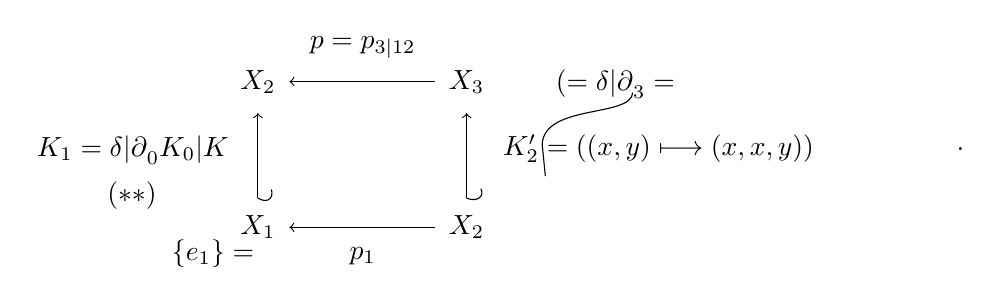
\begin{tikzpicture}[x=1cm,y=1cm]
\node at (-1.60,-1.45) {$(**)$};
\node at (0,0) {$X_2$}; \node at (2.65,0) {$X_3$};
\node at (0,-1.85) {$X_1$}; \node at (-.57,-2.18) {$\{e_1\}=$};
\node at (2.65,-1.85) {$X_2$};
\draw[->] (2.25,0)--(.40,0); \node at (1.33,.43) {$p=p_{\unsure{3|1}2}$};
\draw[->] (0,-1.48)--(0,-.40); \draw(0,-1.48)..controls(.14,-1.56)and(.20,-1.46)..(.17,-1.37);
\node[anchor=east] at (-.25,-.87) {$K_1=\unsure{\delta|\partial}_0\deleted{\unsure{K_0|K}}$};
\draw[->] (2.65,-1.48)--(2.65,-.40); \draw(2.65,-1.48)..controls(2.80,-1.54)and(2.88,-1.44)..(2.83,-1.36);
\draw[->] (2.25,-1.85)--(.40,-1.85); \node at (1.33,-2.22) {$p_1$};
\node[anchor=west] at (2.99,-.85) {$K'_2=((x,y)\longmapsto(x,x,y))$};
\node[anchor=west] at (3.66,-.03) {\inserted{$(=\unsure{\delta|\partial}_3=$}};
\draw(4.76,-.14)..controls(4.74,-.46)and(3.63,-.28)..(3.61,-.80)--(3.65,-1.20);
\node[anchor=west] at (8.75,-.85) {.};
\end{tikzpicture}}

sont-ils cartésiens ? On a $\unsure{\delta|\partial}_3(x,y)=(x,x,y)\deleted{\unsure{=}}$,
\[
\deleted{d\sigma(x,y}\quad d\sigma(x,y)=d(y,x)=(y,x,x)=\deleted{\unsure{\rho}}\rho^2\unsure{\delta|\partial}_3(x\,y)
\]
i.e. $\unsure{\delta|\partial}_3=\rho^{\deleted{\unsure{2}}}d\sigma$.

Donc en général (supposant seulement $\operatorname{card}X_1=1$ i.e. $X_1=\{e_1\}$), \deleted{\unsure{et quand}} pour les, quand a-t-on, \inserted{pour} $\unsure{\zeta|\xi},\unsure{\zeta'|\xi'}\in X_2$,
\[
d(\unsure{\zeta|\xi})=\rho^{\deleted{\unsure{2}}}d
\begin{array}[t]{@{}c@{}}
\sigma(\unsure{\zeta'|\xi'})\\[-1.15ex]
\rule{.3pt}{.6ex}\rule{2.15cm}{.3pt}\rule{.3pt}{.6ex}\\[-.4ex]
\unsure{\zeta''|\xi''}
\end{array}
\quad ?
\]

Il f et s. qu'on ait \deleted{\unsure{alors}}
$\unsure{\zeta|\xi}=\unsure{\zeta''|\xi''}=e_2$,
\margin{d'où $\unsure{\zeta'|\xi'}=e_2$}
\makebox[0pt][l]{\begin{tikzpicture}[baseline=0pt,x=1cm,y=1cm]
\draw(-.14,-.37)..controls(-.62,.26)and(-.62,.66)..(-.33,.74)--(2.62,1.21);
\end{tikzpicture}}\deleted{donc}\quad OK.

\deleted{$\unsure{\zeta|\xi}=\unsure{\zeta'|\xi'}=e_2$ \unsure{ce}} cas est bien cartésien, sans autre hypothèse. Le cas \unsure{du|de} \unsure{$(**)$} s'écrit

\[
p_{\deleted{\unsure{12}}}^{-1}(e_2)\overset{?}=\unsure{\delta|\partial}_3(X_2)\quad[=\rho d\sigma(X_2)=\rho d(X_2)]
\]

\deleted{Mais $\unsure{p_{31}(x,y,z)}=\unsure{(z,x)}=
\underset{\inserted{\unsure{(z,x,y)}}}{\unsure{p\rho(x,y,z)|p\rho^2(x,y,z)}}$
\unsure{i.e.} $\unsure{p_{31}=p\rho|p_{31}=p\rho^2}$,}

\deleted{\unsure{puis}} i.e.
\[
p^{-1}(e_2)\overset{?}=\rho d(X_2)\qquad(\text{on a a priori }\supset)
\]

Si $X_3=X'_3\overset{\mathrm{def}}=\unsure{\mathcal G_3|\mathfrak S_3}\cdot d(X_2)$,
\deleted{\unsure{alors un objet de} $\unsure{X_3}$}
\inserted{l'on est ramené à}
\deleted{$X'_3$ \unsure{s'écrit}} \deleted{\unsure{a|à}} prouvons que \deleted{\unsure{donc}} \unsure{si|$2^\circ$} $\unsure{\zeta|\xi}\in X'_3\setminus\{e_3\}$ satisfait à $p(\unsure{\zeta|\xi})=e_2$, on a $\unsure{\zeta|\xi}\in\rho d(X_2)$. Or $\unsure{\zeta|\xi}$ s'écrit canoniquement
\[
\unsure{\zeta|\xi}=\rho^i d(\eta),\quad\text{avec }\eta\in X_2^*,\quad\text{et }i\in\{0,1,2\},
\]
et on a

\[
p\unsure{\zeta|\xi}=\begin{cases}
\eta\ (\ne e_2)&\text{si }i=0\\
\sigma\eta\ (\ne e_2)&\text{si }i=1
\end{cases}
\]

\deleted{$\unsure{(p\sigma_3d)(x,y)}=\unsure{p\rho d(x,y)}=\unsure{\mathrm{id}}$}

donc $p\unsure{\zeta|\xi}=e_2\Longrightarrow i=1$, \unsure{Qed|qed}
\margin{24}

\scanpage{27}
\mspage{1}

\uline{Structures \unsure{Stratifiées|stratifiées}.}

1. \uline{La situation la plus élémentaire}, en un sens qui apparaîtra, sera la suivante. On se donne des espaces (disons !\unsure{)|\}} en attendant que \unsure{ça|ce} \unsure{deviennent|devienne} des topos\ldots)

(1)
\diagram{\begin{tikzcd}[ampersand replacement=\&]
Y\arrow[r,hook]\&X
\end{tikzcd}}

$Y$ fermé dans $X$. On suppose que la ``structure normale\unsure{''} de $X$ le long de $Y$ soit loc. triviale''\unsure{)|\}} i.e. que pour tout $y\in Y$, existe un voisinage ouvert $X'$ de $y$ et un espace $Z$. pointé par $z$, et un diagramme commutatif (où $Y'=Y\cap X'$)

(2)
\diagram{\begin{tikzcd}[ampersand replacement=\&,column sep=large,row sep=large]
Y'\arrow[r,hook,line width=.8pt]\arrow[d,"\mathrm{can}"',"\wr"]\&X'\arrow[d,"\wr"]\\
Y'\times\{z\}\arrow[r,hook,"\mathrm{id}_{Y'}\times i_{z,Z}"']\&Y'\times Z
\end{tikzcd}}

où $X'\xrightarrow{\sim}Y'\times Z$ est un homéomorphisme.

On considère alors ``le voisinage tubulaire'' (``infinitésimal\unsure{''|'}) de $\unsure{Y|Y'}$ dans $X$, soit

(3)
\diagram{\begin{tikzcd}[ampersand replacement=\&]
Y\arrow[r,hook,line width=.8pt]\&\mathcal V_{Y,X}\arrow[r,hook]\&X
\end{tikzcd}},

dont il faudra donner une définition

\margin{26}

\scanpage{28}

techniquement \unsure{simple|souple}. Si $X$ est \deleted{\unsure{paracompact}} \inserted{un} espace paracompact, on pourra prendre (à titre provisoire !) pour $\mathcal V_{Y,X}$ le ``germe \unsure{d'espaces|d'espace}'' de $X$ autour de $Y$ -- qui est donc un topos, sav. la $\varprojlim$ toposique des voisinages ouverts de $Y$ dans $X$. Intuitivement, $\mathcal V_{Y,X}\hookrightarrow X$ a les propriétés d'une imm. ouverte, et $Y\hookrightarrow\unsure{\mathcal V_{Y,X}|\deleted{\mathcal V}_{Y,X}}$ celles d'une immersion fermée, et (3) constitue une factorisation canonique de (1).

% The cancellation has a long top stroke, an open right side, a stepped lower-left edge and four diagonals; the words remain ordinary transcribed text.
\deleted{L'hypothèse de locale trivialité normale implique que l'on a (moyennant des conditions de ``modération'' convenables) une inclusion}

\margin{L'intérêt principal de cette factorisation, c'est que \unsure{l'inclusion}''
\begin{tikzcd}[ampersand replacement=\&,column sep=small,cramped]
Y\arrow[r,-,to path={(\tikztostart)--(\tikztotarget) node[circle,fill=black,inner sep=.45pt] {} \tikztonodes}]\&\mathcal V_{Y,X}
\end{tikzcd}
est une équivalence d'homotopie'' (indépendamment de toute hyp. de locale trivialité)}

(4)
\diagram{\begin{tikzcd}[ampersand replacement=\&]
Y\arrow[r,"\text{équiv. d'homotopie}"]\&\mathcal V_{Y,X}
\end{tikzcd}}

Supposons p. ex. $Y$ et $X-Y=X^*$ \deleted{des} variétés, et $Z\inserted{{}^*=Z\setminus\{z\}}$ une variété (moyennant des hyp. de modération, l'hyp. sur $Z$ devrait être une conséquence de la première hypothèse), \deleted{\unsure{$Z^*$ est|et que}} alors que $z$ est un pt singulier \inserted{de $Z$}, i.e. $X$ est ``singulier le long de $Y$''. Il est naturel alors de vouloir \unsure{réconstituer|reconstituer} $X$ en termes des variétés $Y$ et $X^*$,

\margin{27}

\scanpage{29}
\mspage{2}

jouant le rôle de ``pierres de construction'' élémentaires. Ceci amène \unsure{à|:} introduire
\[
(5)\qquad \mathcal V_{Y,X}^*\overset{\mathrm{def}}=\mathcal V_{Y,X}\cap X^*=\mathcal V_{Y,X}\setminus Y
\]
\[
(X^*=X-Y),
\]
et le diagramme \unsure{\deleted{un}|---}

\figure{\begin{tikzpicture}[x=.008cm,y=.008cm,every node/.style={inner sep=0pt}]
\node[anchor=base] at (45,-125) {$(6)$};
\node[anchor=base] at (500,-145) {$\mathcal V_{Y,X}^*$};
\node[anchor=base] at (860,-140) {$\mathcal V_{Y,X}$};
\node[anchor=base] at (495,-375) {$X^*$};
\node[anchor=base] at (890,-375) {$X$};
\node[anchor=base west] at (635,-28) {bouchage de trous};
\node[anchor=base west] at (635,-66) {le long de $Y$};
\draw[line width=.55pt] (653,-101) .. controls (642,-101) and (635,-108) .. (633,-117) -- (777,-112);
\draw[line width=.55pt] (633,-117) .. controls (680,-120) and (730,-115) .. (777,-116);
\draw[line width=.7pt] (760,-101) -- (777,-112) -- (762,-125);
\draw[line width=.5pt] (494,-187) -- (493,-288);
\draw[line width=.8pt] (486,-281) -- (493,-289) -- (498,-279);
\draw[line width=.45pt] (886,-183) .. controls (889,-220) and (889,-250) .. (891,-280);
\draw[line width=.65pt] (883,-274) -- (891,-282) -- (898,-273);
\draw[line width=.45pt] (638,-358) -- (808,-358);
\draw[line width=.6pt] (799,-365) -- (811,-358) -- (801,-351);
\end{tikzpicture}}

Je vais regarder (indépendamment de toute hypothèse $=$ de locale trivialité normale, ou de lissité de $X^*$ et $Y$) $X$ comme obtenu par \uline{recollement} de $\mathcal V_{Y,X}$ et de $X^*$ suivant leur intersection $\mathcal V_{Y,X}^*$, ou (en termes plus techniques) comme la somme amalgamée, ou comme \deleted{\unsure{espace|en}} espace ou topos $\varinjlim$ du diagramme \unsure{:}

\figure{\begin{tikzpicture}[x=.008cm,y=.008cm,every node/.style={inner sep=0pt}]
\node[anchor=base] at (45,-195) {$(7)$};
\node[anchor=base] at (565,-175) {$\mathcal V_{Y,X}^*$};
\node[anchor=base] at (905,-170) {$\mathcal V_{Y,X}$};
\node[anchor=base] at (555,-365) {$X^*$};
\draw[line width=.45pt] (690,-137) .. controls (683,-136) and (676,-143) .. (677,-148) -- (809,-150);
\draw[line width=.75pt] (801,-141) -- (811,-150) -- (802,-159);
\draw[line width=.45pt] (549,-205) .. controls (553,-243) and (552,-272) .. (550,-300);
\draw[line width=.65pt] (541,-291) -- (550,-300) -- (557,-290);
\end{tikzpicture}}

\margin{28}

\scanpage{30}

Si on dispose d'une théorie suffisamment souple des types d'homotopie, on devrait pouvoir en déduire le type d'homotopie de $X$ comme ``somme amalgamée'' des types d'homotopie des trois \deleted{\unsure{types|topos}}\inserted{``espaces''} $\mathcal V_{Y,X}^*$, $\mathcal V_{Y,X}$ et $X^*$ (dont les deux premiers sont de nature ``infinitésimale''). Par exemple, on doit avoir pour les espaces déduits en ``tuant les $\Pi_i$ pour $i\geq2$'' -- donc, essentiellement, pour les groupoïdes fondamentaux, un ``théorème de van Kampen'', qui s'exprime par le fait que le diagramme des groupoïdes fondamentaux

\diagram{\begin{tikzpicture}[x=0.008cm,y=-0.008cm,line width=0.45pt,line cap=round,line join=round]
\node at (62,150) {$(8)$};
\node at (508,104) {$\Pi_1\mathcal V_{Y,X}^*$};
\node at (938,104) {$\Pi_1\mathcal V_{Y,X}$};
\node at (1245,100) {$\bigl(\overset{\approx}{\leftarrow}\Pi_1Y\bigr)$};
\node at (477,341) {$\Pi_1X^*$};
\node at (963,345) {$\Pi_1X$};
\node at (723,52) {$p$};
\node at (410,227) {$i$};
% One short upturned terminal on the upper shaft.
\draw (692,106) -- (775,105) -- (773,99);
% The left vertical ends in a small rounded foot, not a supplied chevron.
\draw (464,194) -- (468,280) .. controls (462,278) and (462,289) .. (468,285) -- (476,279);
% Six separate vertical marks, followed by the shallow curved terminal.
\draw (921,177) -- (923,182);
\draw (924,192) -- (924,196);
\draw (923,211) -- (923,213);
\draw (923,222) -- (923,226);
\draw (923,240) -- (923,244);
\draw (925,256) -- (927,259);
\draw (918,267) .. controls (920,281) and (931,284) .. (940,268);
% The lower parentheses enclose the broken shaft and its target.
\node[transform shape,xscale=1.7,yscale=2.7] at (650,350) {$($};
\node[transform shape,xscale=1.7,yscale=3.9] at (1117,335) {$)$};
% Five separate lower dashes and a detached rightward terminal.
\draw (679,348) -- (689,349);
\draw (711,348) -- (715,348);
\draw (730,347) -- (734,347);
\draw (760,346) -- (769,346);
\draw (797,346) -- (812,346);
\draw (843,339) .. controls (855,345) and (858,347) .. (843,354);
\end{tikzpicture}}

\margin{29}

\scanpage{31}

\mspage{3}
est cocartésien -- ou encore, si $Y,X,X^*$
sont connexes, et qu'on \unsure{choisisse|choisit} un ``pt base'' \begin{tikzpicture}[baseline=0pt,x=1cm,y=1cm]
\path[use as bounding box] (0,-.02) rectangle (.56,.72);
\draw[line width=.35pt] (0,.02) .. controls (.07,.26) and (.35,.43) .. (.47,.60);
\node[inner sep=0pt] at (.20,.67) {$\unsure{\wedge|x}$};
\end{tikzpicture} de $\Pi_1\mathcal V_{Y,X}^*$ (i.e. par définition, un rev. universel de $\mathcal V_{Y,X}^*$) (d'où \deleted{des}
pts bases de $\Pi_1\mathcal V_{Y,X}$, \begin{tikzpicture}[baseline=(old.base),x=1cm,y=1cm]
\node[anchor=base west,inner sep=0pt] (old) at (0,0) {\deleted{\unsure{et un point}}};
\node[anchor=base west,inner sep=0pt] at (-.18,.48) {\inserted{$\Pi_1X^*,\Pi_1X)$}};
\node[anchor=base west,inner sep=0pt] at (2.75,.40) {\deleted{de $\Pi_1X^*)$}};
\end{tikzpicture}, qu'on a un isom. \begin{tikzpicture}[baseline=0pt,x=1cm,y=1cm]
\path[use as bounding box] (0,-.02) rectangle (1.20,.73);
\draw[line width=.35pt] (.02,.02) .. controls (.13,.22) and (.65,.34) .. (1.02,.40);
\node[anchor=base west,inner sep=0pt] at (.23,.49) {\inserted{can.}};
\end{tikzpicture} de groupes fonda-\\
mentaux

\[
(9)\qquad \Pi_1(X)\simeq\Pi_1(X^*)\wedge_{\Pi_1\mathcal V_{Y,X}^*}
\begin{tikzpicture}[baseline=(v.base)]
\node[inner sep=0pt] (v) at (0,0) {$\Pi_1(\mathcal V_{Y,X})$};
\draw[line width=.35pt] ([yshift=-.04cm]v.south west) -- ([yshift=-.19cm]v.south west) -- ([yshift=-.19cm]v.south east) -- ([yshift=-.04cm]v.south east);
\node[anchor=north,inner sep=0pt] at ([yshift=-.27cm]v.south) {$\simeq\Pi_1(Y)$};
\end{tikzpicture},
\]

où $\Pi_1(\mathcal V_{Y,X})$ est isom. \begin{tikzpicture}[baseline=0pt,x=1cm,y=1cm]
\path[use as bounding box] (0,-.02) rectangle (2.95,.80);
\draw[line width=.35pt] (.02,.02) .. controls (.12,.27) and (.55,.36) .. (.95,.42);
\node[anchor=base west,inner sep=0pt] at (.22,.48) {\inserted{extérieurem\textsuperscript{t}}};
\end{tikzpicture} à $\Pi_1(Y)$.

\deleted{\unsure{relatif} à un pt base choisi de}

Pour expliciter $\Pi_1(X)$ en termes des
données ``élémentaires'', \deleted{il reste} dont $\Pi_1(Y)$ \begin{tikzpicture}[baseline=0pt,x=1cm,y=1cm]
\path[use as bounding box] (0,-.02) rectangle (1.00,.65);
\node[anchor=base west,inner sep=0pt] at (.08,.37) {\inserted{et}};
\draw[line width=.35pt] (.02,.22) -- (1.00,.22);
\end{tikzpicture}
$\Pi_1(X^*)$, \unsure{\deleted{et}|et} il \begin{tikzpicture}[baseline=(word.base),x=1cm,y=1cm]
\node[anchor=base west,inner sep=0pt] (word) at (0,0) {resterait};
\draw[line width=.35pt] (1.03,-.14) .. controls (1.00,.12) and (1.60,.24) .. (1.72,.52);
\end{tikzpicture} encore à expliciter la structure de $\Pi_1(\mathcal V_{Y,X}^*)$, qui s'envoie dans l'un et dans l'autre, donnant lieu justement au diagramme

\diagram{\begin{tikzpicture}[x=1cm,y=1cm]
\node[inner sep=0pt] at (-2.65,-.88) {$(10)$};
\node[inner sep=0pt] (a) at (0,0) {$\Pi_1(\mathcal V_{Y,X}^*)$};
\node[inner sep=0pt] (b) at (4.05,0) {$\Pi_1(\deleted{\unsure{X}}Y)$};
\node[inner sep=0pt] (c) at (0,-2.05) {$\Pi_1(X^*)$};
\draw[->,line width=.45pt] (a.east) -- (b.west);
\draw[->,line width=.45pt] (a.south) -- (c.north);
\node[anchor=south west,inner sep=0pt,align=left,font=\small] at (2.85,.65) {cette flèche définie \unsure{moy\textsuperscript{t}}\\
\unsure{d'un choix|des choix} suppl. (pt base de $Y$\\
et classe de chemins de\\
$x$ vers $y$};
\draw[line width=.35pt] (2.63,1.04) .. controls (2.25,1.03) and (2.12,.76) .. (2.12,.49);
\node[inner sep=0pt] at (2.10,.29) {$\cdot$};
\node[inner sep=0pt] at (2.08,.18) {$\cdot$};
\end{tikzpicture}}

qui exprime (8). C'est ici que l'hypothèse

\margin{30}

\scanpage{32}

de \uline{locale trivialité normale} a un rôle à jouer (celle de lissité \unsure{restant} comme devant techniquement inutile \deleted{\unsure{)|?}}, son rôle était plutôt de nature heuristique ...).

\deleted{\unsure{On}} On doit se débrouiller, dans ce cas, pour démontrer que les propriétés homo-
topiques de l'inclusion
\begin{tikzcd}[ampersand replacement=\&,cramped,column sep=small]
\mathcal V^*_{Y,X}\arrow[r,-,to path={(\tikztostart) ++(.1,.07) .. controls +(-.13,.06) and +(-.13,0) .. ++(0,-.07) -- (\tikztotarget) \tikztonodes}]\&\mathcal V_{Y,X}
\end{tikzcd}
\margin{\diagram{\begin{tikzcd}[ampersand replacement=\&,row sep=small]
{}\\
Y\arrow[u,hook',"{\substack{\text{homo-}\\\text{topisme}}}","{\text{\deleted{\unsure{Id}}}}"']
\end{tikzcd}}}
sont celles d'une \uline{fibration} \uline{localement triviale de fibre} $\mathcal V^*_{z,Z}$ :

\noindent (11) $\mathcal V^*_{Y,X}\longrightarrow\mathcal V_{Y,X}$ est une ``fibration homotopique'' de fibre $\mathcal V^*_{z,X}$, de base
\begin{tikzcd}[ampersand replacement=\&,cramped,column sep=4em]
Y\arrow[r,-,"{\approx\,\mathrm{homot}}",to path={(\tikztostart) ++(.1,.055) .. controls +(-.12,.05) and +(-.12,0) .. ++(0,-.055) -- (\tikztotarget) (\tikztostart) ++(.33,0) -- ++(.12,-.025) -- ++(.16,.025) (\tikztotarget) ++(-.01,.04) .. controls +(.06,0) and +(.06,0) .. ++(0,-.08) \tikztonodes}]\&\mathcal V_{Y,\unsure{\lambda|X}}
\end{tikzcd}

--- et c'est cela qui devrait même, dans le contexte toposique (p. ex. celui des schémas avec la top. étale) servir de \uline{définition} de la ``locale
\begin{tikzpicture}[baseline=(normalebase.base)]
\node[anchor=base west,inner sep=0pt] (normalebase) at (0,0) {trivialité};
\node[anchor=south east,inner sep=0pt,font=\footnotesize] at ([xshift=.05cm,yshift=.30cm]normalebase.north east) {\inserted{normale}};
\draw ([xshift=-.55cm,yshift=.20cm]normalebase.north east) -- ([xshift=-.25cm,yshift=.20cm]normalebase.north east) .. controls ([xshift=.02cm,yshift=.20cm]normalebase.north east) and ([xshift=.03cm,yshift=-.06cm]normalebase.north east) .. ([xshift=.06cm,yshift=-.15cm]normalebase.north east) -- ([xshift=.39cm,yshift=.08cm]normalebase.north east) .. controls ([xshift=.50cm,yshift=.14cm]normalebase.north east) and ([xshift=.52cm,yshift=.20cm]normalebase.north east) .. ([xshift=.48cm,yshift=.25cm]normalebase.north east);
\end{tikzpicture}
homotopique'' de l'inclusion
\begin{tikzcd}[ampersand replacement=\&,cramped,column sep=small]
Y\arrow[r,-,to path={(\tikztostart) ++(.1,.07) .. controls +(-.13,.06) and +(-.13,0) .. ++(0,-.07) -- (\tikztotarget) (\tikztotarget) ++(0,.04) -- ++(0,-.08) \tikztonodes}]\&X
\end{tikzcd}.

(Bien sûr, dans le contexte schématique, il faudra de plus travailler avec des types d'homotopie profinis, et même
\begin{tikzpicture}[baseline=(localiserbase.base)]
\node[anchor=base west,inner sep=0pt] (localiserbase) at (0,0) {``localiser''};
\node[anchor=south west,inner sep=0pt,font=\footnotesize] at ([xshift=-.20cm,yshift=.30cm]localiserbase.north west) {\inserted{sans doute}};
\draw ([xshift=-.04cm,yshift=-.03cm]localiserbase.north west) .. controls ([xshift=-.03cm,yshift=.17cm]localiserbase.north west) and ([xshift=.12cm,yshift=.25cm]localiserbase.north west) .. ([xshift=.36cm,yshift=.23cm]localiserbase.north west) .. controls ([xshift=.64cm,yshift=.18cm]localiserbase.north west) and ([xshift=.84cm,yshift=.12cm]localiserbase.north west) .. ([xshift=1.04cm,yshift=.23cm]localiserbase.north west);
\end{tikzpicture}
ces types d'homotopie

\margin{31}

\scanpage{33}
\mspage{4}

en l'ens. des nbs premiers qui sont distincts des caractéristiques résiduelles qui interviennent, vu que ce n'est que dans ce contexte modifié que l'on peut prouver des théorèmes qu'il faut \deleted{de trivialité}, cf Artin-Mazur ...).

On aura en particulier une suite exacte d'homotopie \deleted{\unsure{longue}} (choisissant un \deleted{``\unsure{pt base}''} ``pt base'' dans une série convenable \deleted{\unsure{p}} des germes d'espace $\mathcal V^*_{z,Z}$) :

\diagram{\begin{tikzpicture}[x=0.0095cm,y=-0.0095cm,font=\small,line width=0.45pt,line cap=round,line join=round]
\node at (42,105) {$(1\unsure{2|1})$};
\node at (250,86) {$\ldots$};
\node at (426,75) {$\Pi_i(\mathcal V^*_{\unsure{\deleted{Z}z|z|Z},Z})$};
\node at (762,67) {$\Pi_i(\mathcal V^*_{Y,X})$};
\node at (1006,66) {$\Pi_i(Y)$};
\node at (1248,70) {$\Pi_{i-1}(\mathcal V^*_{z,Z})$};
% The first connector has two wings; the next two have only short terminal returns.
\draw (560,69) -- (621,65);
\draw (615,60) -- (621,65) -- (615,72);
\draw (902,64) -- (939,64) -- (938,61);
\draw (1083,72) -- (1123,72) -- (1121,68);
% The terminal shaft and the visible clipped ellipsis fragment are not completed past the scan.
\draw (1368,73) -- (1393,76) -- (1393,80);
\node at (1407,75) {$\cdot$};
\node at (1427,78) {$-$};
\node at (1415,132) {,};
\end{tikzpicture}}

qui nous intéresse surtout en basses dimensions

\diagram{\begin{tikzpicture}[x=0.0095cm,y=-0.0095cm,font=\small,line width=0.45pt,line cap=round,line join=round]
\node at (48,100) {$(13)$};
\node at (295,88) {$\Pi_2(Y)$};
\node at (505,82) {$\Pi_1(\mathcal V^*_{z,Z})$};
\node at (796,68) {$\Pi_1(\mathcal V^*_{Y,X})$};
\node at (1059,78) {$\Pi_1(Y)$};
\node at (1288,75) {$\Pi_0(\mathcal V^*_{z,Z})$};
\node at (1296,264) {$\Pi_0(\mathcal V^*_{Y,X})$};
\node at (1278,422) {$\Pi_0(Y)$};
% Two incomplete rightward terminals, then two complete rightward heads.
\draw (366,83) -- (409,78) -- (405,75);
\draw (609,78) -- (670,77) -- (669,72);
\draw (920,77) -- (978,77);
\draw (971,70) -- (978,77) -- (971,84);
\draw (1146,74) -- (1193,74);
\draw (1188,69) -- (1193,74) -- (1188,79);
% Both downward shafts have visible terminal heads.
\draw (1265,130) -- (1269,207);
\draw (1262,200) -- (1269,207) -- (1274,201);
\draw (1281,312) -- (1284,374);
\draw (1279,369) -- (1284,374) -- (1288,369);
\node at (913,140) {$\underbrace{\hspace{3.83cm}}$};
% Additional small pen loop over the left part of the brace.
\draw (735,147) .. controls (754,133) and (778,132) .. (785,148);
\node at (928,192) {qui intervient dans $(10)$};
\end{tikzpicture}}

Si on suppose p. ex. que $z$ ne disconnecte pas $Z$ localement i.e. : \deleted{\unsure{donc}} la ``fibre $\mathcal V^*_{z,Z}$ est conne\unsure{x}
% The final cluster of the preceding word meets the paper/scan edge.
(ou encore, que $Y$ ne disconnecte pas $X$ loc\textsuperscript{t}.), alors $\Pi_1(\mathcal V^*_{Y,X})$ est une \uline{extension} de $\Pi_1(Y)$ par un quotient de $\Pi_1(\mathcal V^*_{z,Z})$, \deleted{\unsure{et}}

\margin{32}

\scanpage{34}

(savoir le quotient par l'image de $\Pi_2(Y)$),
et $=$ par $\Pi_1(\mathcal V^*_{z,Z})$ lui-$=$ si $\Pi_2(Y)$ est
nul. Si on suppose pour simplifier\\
\hspace{.25cm}{\small\deleted{\unsure{cyclique}}}\\[-.35em]
que $\Pi_2(Y)\begin{tikzpicture}[baseline=-.35ex,x=1cm,y=1cm]
\draw[line width=.35pt] (0,0) -- (.53,.01) -- (.56,.055) -- (.60,-.035);
\end{tikzpicture}\Pi_1(\mathcal V^*_{z,Z})$ est nul, on trouve
donc un diagramme qui précise (10)

\diagram{\begin{tikzpicture}[x=.8cm,y=.9cm]
\node[inner sep=0pt] (one) at (0,0) {$1$};
\node[inner sep=0pt] (fibre) at (2.3,0) {$\Pi_1(\mathcal V^*_{z,Z})$};
\node[inner sep=0pt] (middle) at (5.7,0) {$\Pi_1(\mathcal V^*_{Y,X})$};
\node[inner sep=0pt] (base) at (8.8,0) {$\Pi_1(Y)$};
\node[inner sep=0pt] (last) at (10.4,0) {$1$};
\draw[line width=.45pt] (one.east) -- ([xshift=-.18cm]fibre.west);
\draw[line width=.45pt] ([xshift=-.18cm]fibre.west) -- ([xshift=-.26cm,yshift=.13cm]fibre.west);
\draw[line width=.45pt] (fibre.east) -- ([xshift=-.15cm]middle.west);
\draw[line width=.45pt] ([xshift=-.15cm,yshift=.04cm]middle.west) -- ([xshift=-.15cm,yshift=-.04cm]middle.west);
\draw[->,line width=.45pt] (middle.east) -- (base.west);
\draw[line width=.45pt] (base.east) -- (last.west);
\node[inner sep=0pt] (bottom) at (5.7,-2.12) {$\Pi_1(X^*)$};
\draw[->,line width=.45pt] ([yshift=-.20cm]middle.south) -- ([yshift=.05cm]bottom.north);
\node[inner sep=0pt] at (2.25,-.48) {$\Vert$};
\node[inner sep=0pt] at (2.3,-1.00) {$(I\ \text{``inertie''})$};
\node[inner sep=0pt,rotate=45] at (6.95,-.46) {$\Vert$};
\node[inner sep=0pt,anchor=west] at (6.85,-1.00) {$(D\ \text{``décomposition''})$};
\node[inner sep=0pt] at (2.3,.78) {$\deleted{\unsure{\Pi_1|\pi_1}}$};
\node[inner sep=0pt] at (.83,-.25) {$\deleted{\unsure{(14)}}$};
\node[inner sep=0pt] at (-1.45,-1.55) {$(14)$};
\node[inner sep=0pt] at (12.4,-2.80) {,};
\end{tikzpicture}}

où la ligne horizontale est exacte.

Un cas intéressant est celui où les
``pièces de construction'' qui \deleted{\unsure{sont}} interviennent,
savoir $Y$, $X^*$ et $\mathcal V^*_{Z,z}$, sont des espaces
``$K(\Pi,1)$'', i.e.
\[
(15)\qquad \Pi_i(Y),\ \Pi_i(X^*),\ \Pi_i(\mathcal V^*_{Z,z}]\quad\text{nuls pour }i\geq 2,
\]
alors on en déduit qu'il en est de $=$
pour $\mathcal V^*_{Y,X}$ (et bien sûr pour $\mathcal V^*_{Y,X}\begin{tikzpicture}[baseline=0pt,x=1cm,y=1cm]
\path[use as bounding box] (-.42,-.05) rectangle (.63,.72);
\draw[<-,line width=.35pt] (-.36,0) -- (.36,0);
\node[inner sep=0pt] at (0,.25) {$\approx$};
\node[inner sep=0pt] at (.22,.58) {$\mathrm{homot.}$};
\end{tikzpicture}Y$).
Si on a la ``\unsure{théorie|Théorie} souple des \uline{liens} des
types d'homotopie'' à laquelle je faisais

\margin{33}

\scanpage{35}\mspage{5}

allusion, on devrait pouvoir \begin{tikzpicture}[baseline=(alorsb.base)]
\node[anchor=base west,inner sep=0pt] (alorsb) at (0,0) {exprimer};
\node[anchor=south east,inner sep=0pt,font=\footnotesize] at ([xshift=.05cm,yshift=.30cm]alorsb.north east) {\inserted{alors}};
\draw ([xshift=-.52cm,yshift=.20cm]alorsb.north east) .. controls ([xshift=.03cm,yshift=.20cm]alorsb.north east) and ([xshift=.05cm,yshift=-.04cm]alorsb.north east) .. ([xshift=.06cm,yshift=-.15cm]alorsb.north east) -- ([xshift=.43cm,yshift=.23cm]alorsb.north east);
\end{tikzpicture}
le \uline{type d'homotopie} \uline{de} $\deleted{\unsure{Z}}X$ (et non seulement son $\Pi_1$) en termes du \begin{tikzpicture}[baseline=(groupb.base)]
\node[anchor=base west,inner sep=0pt] (groupb) at (0,0) {diagramme};
\node[anchor=south east,inner sep=0pt,font=\footnotesize] at ([xshift=.47cm,yshift=.36cm]groupb.north east) {\inserted{de groupoïdes}};
\draw ([xshift=.04cm,yshift=-.10cm]groupb.north east) .. controls ([xshift=.14cm,yshift=.22cm]groupb.north east) and ([xshift=.38cm,yshift=.25cm]groupb.north east) .. ([xshift=.67cm,yshift=.26cm]groupb.north east) .. controls ([xshift=.92cm,yshift=.27cm]groupb.north east) and ([xshift=1.03cm,yshift=.31cm]groupb.north east) .. ([xshift=.99cm,yshift=.35cm]groupb.north east);
\end{tikzpicture} (8), ou ce qui revient au $=$, du diagramme de groupes (10).

En tous cas, il est clair (indépendam-
ment de toute hypothèse de nullité de certains $\Pi_i$, ou de locale trivialité normale) comment reconstruire, en termes du diagramme 8, la \begin{tikzpicture}[baseline=(catone.base)]
\node[anchor=base west,inner sep=0pt] (catone) at (0,0) {catégorie};
\node[anchor=south east,inner sep=0pt,font=\footnotesize] at ([xshift=.05cm,yshift=.30cm]catone.north west) {\inserted{\unsure{ss}}};
\node[anchor=south east,inner sep=0pt] at ([xshift=.12cm,yshift=.35cm]catone.north east) {\inserted{$\unsure{\mathcal F|\mathfrak F}$}};
\draw ([xshift=-.12cm,yshift=-.10cm]catone.north west) .. controls ([xshift=-.03cm,yshift=.08cm]catone.north west) and ([xshift=.24cm,yshift=.17cm]catone.north west) .. ([xshift=.27cm,yshift=.33cm]catone.north west);
\draw ([xshift=.04cm,yshift=-.10cm]catone.north east) .. controls ([xshift=.14cm,yshift=.10cm]catone.north east) and ([xshift=.37cm,yshift=.23cm]catone.north east) .. ([xshift=.39cm,yshift=.45cm]catone.north east);
\end{tikzpicture} dans la cat. des faisceaux sur $X$, \deleted{dont} formée des $F$ tels que l'on ait

\[
(16)\qquad F\mid X^*\quad\text{et}\quad F\mid Y\quad\text{localement triviaux}\unsure{,|;}
\]

Cette \begin{tikzpicture}[baseline=(cattwob.base)]
\node[anchor=base west,inner sep=0pt] (cattwob) at (0,0) {catégorie};
\node[anchor=south east,inner sep=0pt,font=\footnotesize] at ([xshift=.12cm,yshift=.34cm]cattwob.north east) {\inserted{$\unsure{\mathcal F|\mathfrak F}$}};
\draw ([xshift=.03cm,yshift=-.10cm]cattwob.north east) .. controls ([xshift=.08cm,yshift=.08cm]cattwob.north east) and ([xshift=.39cm,yshift=.19cm]cattwob.north east) .. ([xshift=.46cm,yshift=.38cm]cattwob.north east);
\end{tikzpicture} est équivalente en effet à celle des systèmes

\[
(17)\qquad (E_{X^*},E_{Y,X}\mathpunct{\begin{tikzpicture}[baseline=-.25ex]
\node[inner sep=0pt] at (.03,.23) {$\cdot$};
\node[inner sep=0pt] at (0,.12) {$\cdot$};
\node[inner sep=0pt] at (.11,-.03) {$,$};
\end{tikzpicture}}\varphi)
\]

\deleted{\unsure{formés}} \begin{tikzpicture}[baseline=(rewriteb.base)]
\node[anchor=base west,inner sep=0pt] (rewriteb) at (0,0) {\deleted{\unsure{d'un}} système};
\node[anchor=south west,inner sep=0pt,font=\footnotesize] at ([xshift=.15cm,yshift=.30cm]rewriteb.north west) {\inserted{où $E_{X^*}$ est un}};
\draw ([xshift=.76cm,yshift=-.04cm]rewriteb.north west) .. controls ([xshift=.79cm,yshift=.14cm]rewriteb.north west) and ([xshift=1.55cm,yshift=.17cm]rewriteb.north west) .. ([xshift=2.15cm,yshift=.29cm]rewriteb.north west) .. controls ([xshift=2.28cm,yshift=.33cm]rewriteb.north west) and ([xshift=2.31cm,yshift=.37cm]rewriteb.north west) .. ([xshift=2.25cm,yshift=.37cm]rewriteb.north west);
\end{tikzpicture} local sur \begin{tikzpicture}[baseline=(coverb.base)]
\node[anchor=base west,inner sep=0pt] (coverb) at (0,0) {$\Pi_1X^*$};
\node[anchor=south west,inner sep=0pt,font=\footnotesize] (covera) at ([xshift=-.2cm,yshift=.58cm]coverb.north east) {\inserted{($\unsure{\leftrightarrow|\Leftrightarrow}$ un rev. \begin{tikzpicture}[baseline=(etaddb.base)]
\node[anchor=base west,inner sep=0pt] (etaddb) at (0,0) {de $X^{\unsure{*|+}}$};
\node[anchor=south east,inner sep=0pt,font=\footnotesize] at ([xshift=.12cm,yshift=.34cm]etaddb.north west) {\inserted{\unsure{étle|ét.le}}};
\draw ([xshift=.03cm,yshift=-.10cm]etaddb.north west) .. controls ([xshift=.08cm,yshift=.08cm]etaddb.north west) and ([xshift=.39cm,yshift=.19cm]etaddb.north west) .. ([xshift=.46cm,yshift=.38cm]etaddb.north west);
\end{tikzpicture})}};
\draw ([xshift=.05cm,yshift=-.03cm]coverb.north east) .. controls ([xshift=.08cm,yshift=.36cm]coverb.north east) and ([xshift=.20cm,yshift=-.10cm]covera.south west) .. ([xshift=.65cm,yshift=-.10cm]covera.south west) -- ([xshift=1.45cm,yshift=-.10cm]covera.south west);
\draw ([xshift=1.49cm,yshift=-.10cm]covera.south west) -- ([xshift=.08cm,yshift=-.04cm]covera.south east) .. controls ([xshift=.28cm,yshift=-.01cm]covera.south east) and ([xshift=.20cm,yshift=.10cm]covera.south east) .. ([xshift=.14cm,yshift=.09cm]covera.south east);
\end{tikzpicture}, $E_{Y,X}$ un syst. local sur \begin{tikzpicture}[baseline=(piaddb.base)]
\node[anchor=base west,inner sep=0pt] (piaddb) at (0,0) {$\Pi_1\mathcal V_{Y,X}$};
\node[anchor=south west,inner sep=0pt,font=\footnotesize] at ([xshift=-.10cm,yshift=.32cm]piaddb.north east) {\inserted{$\xleftarrow{\approx}\Pi_1Y$}};
\draw ([xshift=.06cm,yshift=-.13cm]piaddb.north east) .. controls ([xshift=-.03cm,yshift=.13cm]piaddb.north east) and ([xshift=.35cm,yshift=.20cm]piaddb.north east) .. ([xshift=.98cm,yshift=.42cm]piaddb.north east);
\end{tikzpicture} ($\leftrightarrow$ un rev. ét.le de $Y$) et $\varphi$ un hom. de syst. locaux sur $\Pi_1\mathcal V^*_{Y,\unsure{\lambda|X}}$

\margin{34}
